% \documentclass[12pt,english,ignorenonframetext,aspectratio=169,]{beamer}
\documentclass[11pt,english,ignorenonframetext,]{beamer}

%%%%%%%%%%%%%%%
%% Beamer theme
% choose one from http://deic.uab.es/~iblanes/beamer_gallery/
% or http://www.hartwork.org/beamer-theme-matrix/
% \usetheme{Warsaw}
\usetheme{CambridgeUS}

%%%%%%%%%%%%%%%%%%%%%%
%% Beamer color theme
%% default albatross beaver beetle crane dolphin dove fly lily
%% orchid rose seagull seahorse whale wolverine

%\usecolortheme{seahorse}  %% very lighty
\usecolortheme{dolphin}    %% nice blue
\usecolortheme{orchid}     %% dark red ?
\usecolortheme{whale}      %% black and blue as Warsaw

%%%%%%%%%%%%%%%%%%%%%%%%%%%%%%%%%%%%%%%%%%%%%%%%%%%%%%%%%%%%%%%%%%%%%%%%%%%%%%%%
%% Change the theme
%\setbeamercolor{alerted text}{fg=orange}
%\setbeamercolor{background canvas}{bg=white}
%\setbeamercolor{block body alerted}{bg=normal text.bg!90!black}
%\setbeamercolor{block body}{bg=normal text.bg!90!black}
%\setbeamercolor{block body example}{bg=normal text.bg!90!black}
%\setbeamercolor{block title alerted}{use={normal text,alerted text},fg=alerted text.fg!75!normal text.fg,bg=normal text.bg!75!black}
%\setbeamercolor{block title}{bg=blue}
%\setbeamercolor{block title example}{use={normal text,example text},fg=example text.fg!75!normal text.fg,bg=normal text.bg!75!black}
%\setbeamercolor{fine separation line}{}
\setbeamercolor{frametitle}{fg=black}
%\setbeamercolor{item projected}{fg=black}
%\setbeamercolor{normal text}{bg=black,fg=yellow}
%\setbeamercolor{palette sidebar primary}{use=normal text,fg=normal text.fg}
%\setbeamercolor{palette sidebar quaternary}{use=structure,fg=structure.fg}
%\setbeamercolor{palette sidebar secondary}{use=structure,fg=structure.fg}
%\setbeamercolor{palette sidebar tertiary}{use=normal text,fg=normal text.fg}
%\setbeamercolor{section in sidebar}{fg=brown}
%\setbeamercolor{section in sidebar shaded}{fg= grey}
\setbeamercolor{separation line}{}
%\setbeamercolor{sidebar}{bg=red}
%\setbeamercolor{sidebar}{parent=palette primary}
%\setbeamercolor{structure}{bg=black, fg=green}
%\setbeamercolor{subsection in sidebar}{fg=brown}
%\setbeamercolor{subsection in sidebar shaded}{fg= grey}
%\setbeamercolor{title}{fg=blackblue}
%\setbeamercolor{titlelike}{fg=blackblue}


%%%%%%%%%%%%%%%%%%%%%%%
%% Other beamer options
% \setbeamercovered{transparent}
\setbeamercovered{invisible}
% Permet de laisser en gris le texte qui n'est pas encore apparu (lorsqu'on utilise les commandes avec des <1,2> ou <4-9>.

%\setbeamercolor{normal text}{fg=black,bg=white}

%%%%%%%%%%%%%%%%%%%%%%%
%% Change Beamer fonts
% \usefonttheme{default}
% \usefonttheme[onlymath]{serif}
\usefonttheme{serif}

\setbeamerfont{title}{family=\rm}
\setbeamerfont{titlelike}{family=\rm}
\setbeamerfont{frametitle}{family=\rm}

%%%%%%%%%%%%%%%%%%%%%%%%%%%%%%%%%%%%%%%%%%%%%%%%%%%%%%%%%%%%%%%%%%%%%%%%%%%%%%%%
%% innertheme
%% rectangles circles inmargin rounded
% \useinnertheme{rounded}  % XXX My preference
\useinnertheme{circles}    % XXX

%%%%%%%%%%%%%%%%%%%%%%%%%%%%%%%%%%%%%%%%%%%%%%%%%%%%%%%%%%%%%%%%%%%%%%%%%%%%%%%%
%% outertheme
%% infolines miniframes shadow sidebar smoothbars smoothtree split tree
%\useoutertheme{infolines}

%% No navigation symbol.
\setbeamertemplate{navigation symbols}{}
\beamertemplatenavigationsymbolsempty

% XXX Add a background image to the slides
% \usepackage{tikz}
% \setbeamertemplate{background}{
\includegraphics[width=\paperwidth,height=\paperheight,keepaspectratio]{IETR.jpg}}
% \setbeamertemplate{background}{{\centering\begin{tikzpicture}\node[opacity=0.15]{
\includegraphics[width=0.98\paperwidth]{IETR_et_partenaires_IETR.png}};\end{tikzpicture}}}

% Other options
%\setbeamertemplate{footline}[page number]

\beamertemplateballitem
\setbeamertemplate{itemize item}[square]


\setbeamertemplate{caption}[numbered]
\setbeamertemplate{caption label separator}{: }
\setbeamercolor{caption name}{fg=normal text.fg}
\beamertemplatenavigationsymbolsempty
\usepackage{lmodern}
\usepackage{color}
  \newcommand{\urlb}[1]{\textcolor{blue}{\url{#1}}}
%% Color definition
\usepackage{xcolor}
%% WARNING attention when changing the colors, change both the {RGB}{r,g,b} and % rgb(r,g,b)
\definecolor{blackblue}{RGB}{19,19,59}  % rgb(48,48,150)
\definecolor{bleu}{RGB}{0,0,204}           % rgb(0,0,204)
\definecolor{deeppurple}{RGB}{102,0,204}   % rgb(102,0,204)
\definecolor{darkgreen}{RGB}{0,100,0}      % rgb(0,100,0)
\definecolor{yellowgreen}{RGB}{200,215,0}  % rgb(200,215,0)
\definecolor{bluegreen}{RGB}{0,185,140}    % rgb(0,185,140)
\definecolor{gold}{RGB}{255,180,0}         % rgb(255,180,0)
\definecolor{meca}{RGB}{255,110,0}         % rgb(255,110,0)
\definecolor{strongred}{RGB}{255,0,0}      % rgb(255,0,0)
\definecolor{normalred}{RGB}{204,0,0}      % rgb(204,0,0)
\definecolor{darkred}{RGB}{174,0,0}        % rgb(174,0,0)
\definecolor{info}{RGB}{174,0,0}        % rgb(174,0,0)
\definecolor{darkblue}{RGB}{0,0,174}        % rgb(0,0,174)
\definecolor{maths}{RGB}{0,0,174}        % rgb(0,0,174)
\definecolor{darkpurple}{RGB}{114,0,114}   % rgb(114,0,114)
\definecolor{ml}{RGB}{114,0,114}   % rgb(114,0,114)

\usepackage{amssymb,amsmath}
\usepackage{bbm,bm}  % bold maths symbols
\usepackage{ifxetex,ifluatex}
\usepackage{fixltx2e} % provides \textsubscript

% % FIXME remove as soon as possible, it slows down compilation to import TikZ
% %% TikZ
% \usepackage{tikz}
% \usetikzlibrary{snakes,arrows,shapes}
% % https://tex.stackexchange.com/a/226974/
% \tikzset{
%   font={\fontsize{10pt}{10}\selectfont}
% }
\usepackage{tikzsymbols}  % https://tex.stackexchange.com/a/227226/97964

\IfFileExists{macrosText.sty}{\usepackage{macrosText}}{}

% For algorithms
\usepackage[linesnumbered,commentsnumbered,inoutnumbered,slide]{algorithm2e}


\ifnum 0\ifxetex 1\fi\ifluatex 1\fi=0 % if pdftex
  \usepackage[T1]{fontenc}
  \usepackage[utf8]{inputenc}
\else % if luatex or xelatex
  \ifxetex
    \usepackage{mathspec}
  \else
    \usepackage{fontspec}
  \fi
  \defaultfontfeatures{Ligatures=TeX,Scale=MatchLowercase}
\fi
% use upquote if available, for straight quotes in verbatim environments
\IfFileExists{upquote.sty}{\usepackage{upquote}}{}
% use microtype if available
\IfFileExists{microtype.sty}{%
\usepackage{microtype}
\UseMicrotypeSet[protrusion]{basicmath} % disable protrusion for tt fonts
}{}
\newif\ifbibliography
\hypersetup{
            pdfborder={0 0 0},
            breaklinks=true}
% \urlstyle{same}  % don't use monospace font for urls
% Code embedding.
\usepackage{palatino}              % Use the Palatino font % XXX remove if it is ugly ?
\usepackage{graphicx,grffile}
\makeatletter
\def\maxwidth{\ifdim\Gin@nat@width>\linewidth\linewidth\else\Gin@nat@width\fi}
\def\maxheight{\ifdim\Gin@nat@height>\textheight0.8\textheight\else\Gin@nat@height\fi}
\makeatother
% Scale images if necessary, so that they will not overflow the page
% margins by default, and it is still possible to overwrite the defaults
% using explicit options in \includegraphics[width, height, ...]{}
\setkeys{Gin}{width=\maxwidth,height=\maxheight,keepaspectratio}

\ifxetex
\usepackage{fontspec}
\setmainfont[Ligatures=Historic]{TeX Gyre Pagella}
\newfontfamily\FiraCode{Fira Code}
\setmonofont[Contextuals={Alternate}]{Fira Code}
\newfontfamily\Fontify[Path = ../common/]{Fontify-Regular}
\else
\newcommand{\Fontify}{}
\fi

% Prevent slide breaks in the middle of a paragraph:
\widowpenalties 1 10000
\raggedbottom

% \AtBeginPart{
%   \let\insertpartnumber\relax
%   \let\partname\relax
%   \frame{\partpage}
% }
% \AtBeginSection{
%   \ifbibliography
%   \else
%     \let\insertsectionnumber\relax
%     \let\sectionname\relax
%     \frame{\sectionpage}
%   \fi
% }
% % Si on veut faire apparaître le sommaire courant à chaque nouvelle section.
% \AtBeginSection{
%   \begin{frame}<beamer>%[t]
%   %\frametitle{Local outline}  % Translate the name of the slide
%   \frametitle{\hspace{0pt}}  % Translate the name of the slide
%     \begin{LARGE}  % XXX LARGE font for this slide?
%     \tableofcontents[currentsection, sectionstyle=show/hide, subsectionstyle=hide/hide]
%     \end{LARGE}  % XXX LARGE font for this slide?
%   \end{frame}
% }
% \AtBeginSubsection{
%   \let\insertsubsectionnumber\relax
%   \let\subsectionname\relax
%   \frame{\subsectionpage}
% }

\setlength{\parindent}{0pt}
\setlength{\parskip}{6pt plus 2pt minus 1pt}
\setlength{\emergencystretch}{3em}  % prevent overfull lines
\providecommand{\tightlist}{%
  \setlength{\itemsep}{0pt}\setlength{\parskip}{0pt}}
\setcounter{secnumdepth}{5}

% https://tex.stackexchange.com/a/70495/
\usepackage{appendixnumberbeamer}


% For \justifying command, see https://tex.stackexchange.com/a/148696/
\usepackage{ragged2e}
\addtobeamertemplate{frame begin}{}{\justifying}
\addtobeamertemplate{block begin}{}{\justifying}
\addtobeamertemplate{block alerted begin}{}{\justifying}
\addtobeamertemplate{block example begin}{}{\justifying}
\addtobeamertemplate{itemize body begin}{}{\justifying}
\addtobeamertemplate{itemize item}{}{\justifying}
\addtobeamertemplate{itemize subitem}{}{\justifying}
\addtobeamertemplate{itemize subsubitem}{}{\justifying}
\addtobeamertemplate{enumerate body begin}{}{\justifying}
\addtobeamertemplate{enumerate item}{}{\justifying}
\addtobeamertemplate{enumerate subitem}{}{\justifying}
\addtobeamertemplate{enumerate subsubitem}{}{\justifying}
\addtobeamertemplate{description body begin}{}{\justifying}
\addtobeamertemplate{description item}{}{\justifying}


\title[B-GLR test and Non-Stationary MAB]{The Bernoulli Generalized Likelihood Ratio test (B-GLR) for Non-Stationary Multi-Armed Bandits}
\subtitle{Research Seminar at PANAMA, IRISA lab, Rennes}

\author[Lilian Besson]{\Large \textbf{Lilian Besson}}

\institute[]{{\large
  PhD Student}{\newline
  % \normalsize
  \newline SCEE team, IETR laboratory, CentraleSupélec in Rennes
  \newline \& SequeL team, CRIStAL laboratory, Inria in Lille}}

\date{Thursday $6^{\text{th}}$ of June, $2019$}

\begin{document}
\justifying

\begin{frame}[plain]
  \titlepage

  % XXX manual inclusion of logos
  \begin{center}
    
\includegraphics[height=0.18\textheight]{../common/LogoIETR.png}
    
\includegraphics[height=0.21\textheight]{../common/LogoCS.png}
    
\includegraphics[height=0.18\textheight]{../common/LogoInria.jpg}
  \end{center}

\end{frame}


\begin{frame}{Publications associated with this talk}

  Joint work with my advisor Emilie Kaufmann:

  \begin{itemize}
    \item
      \href{https://hal.inria.fr/hal-02006471/document}{\emph{``Analyse non asymptotique d'un test séquentiel de détection de ruptures et application aux bandits non stationnaires''}}\\
      by \textbf{L. Besson} \&
      \href{http://chercheurs.lille.inria.fr/ekaufman/research.html}{E.
      Kaufmann}

      $\hookrightarrow$ presented at
      \textbf{GRETSI}, in Lille (France), next August 2019

    \vspace*{30pt}

    \item
      \href{https://hal.inria.fr/hal-02006471/document}{\emph{``The Generalized Likelihood Ratio Test meets klUCB: an Improved Algorithm for Piece-Wise Non-Stationary Bandits''}}\\
      by \textbf{L. Besson} \&
      \href{http://chercheurs.lille.inria.fr/ekaufman/research.html}{E.
      Kaufmann}\\
      February 2019,
      pre-print on
      \href{https://hal.inria.fr/hal-02006471}{\textcolor{blue}{HAL-02006471}}
      and
      \href{https://arxiv.org/abs/1902.01575}{\textcolor{blue}{arXiv:1902.01575}}

  \end{itemize}

\end{frame}


\section{\hfill{}Outline of the talk\hfill{}}

\begin{frame}{Outline of the talk}

  \begin{enumerate}
    \item
      (Stationary) Multi-armed bandits problems
    \vspace*{15pt}

    \item
      Piece-wise stationary multi-armed bandits problems
    \vspace*{15pt}

    \item
      The B-GLR test and its finite time properties
    \vspace*{15pt}

    \item
      The BGLR-T + klUCB algorithm
    \vspace*{15pt}

    \item
      Regret analysis
    \vspace*{15pt}

    \item
      Numerical simulations
  \end{enumerate}

\end{frame}


\section{\hfill{}1. (Stationary) Multi-armed bandits problems\hfill{}}

\begin{frame}{1. (Stationary) Multi-armed bandits problems}

  \begin{enumerate}
    \item
    \alert{\textbf{%
      (Stationary) Multi-armed bandits problems
    }}
    \vspace*{15pt}

    \item
    \textcolor{gray}{
      Piece-wise stationary multi-armed bandits problems
    }
    \vspace*{15pt}

    \item
    \textcolor{gray}{
      The B-GLR test and its finite time properties
    }
    \vspace*{15pt}

    \item
    \textcolor{gray}{
      The BGLR-T + klUCB algorithm
    }
    \vspace*{15pt}

    \item
    \textcolor{gray}{
      Regret analysis
    }
    \vspace*{15pt}

    \item
    \textcolor{gray}{
      Numerical simulations
    }
  \end{enumerate}

\end{frame}

\subsection{\hfill{}What is a bandit problem?\hfill{}}

\begin{frame}{Multi-armed bandits}

  $=$ Sequential decision making problems in uncertain environments :

  \begin{center}
    % \centering
    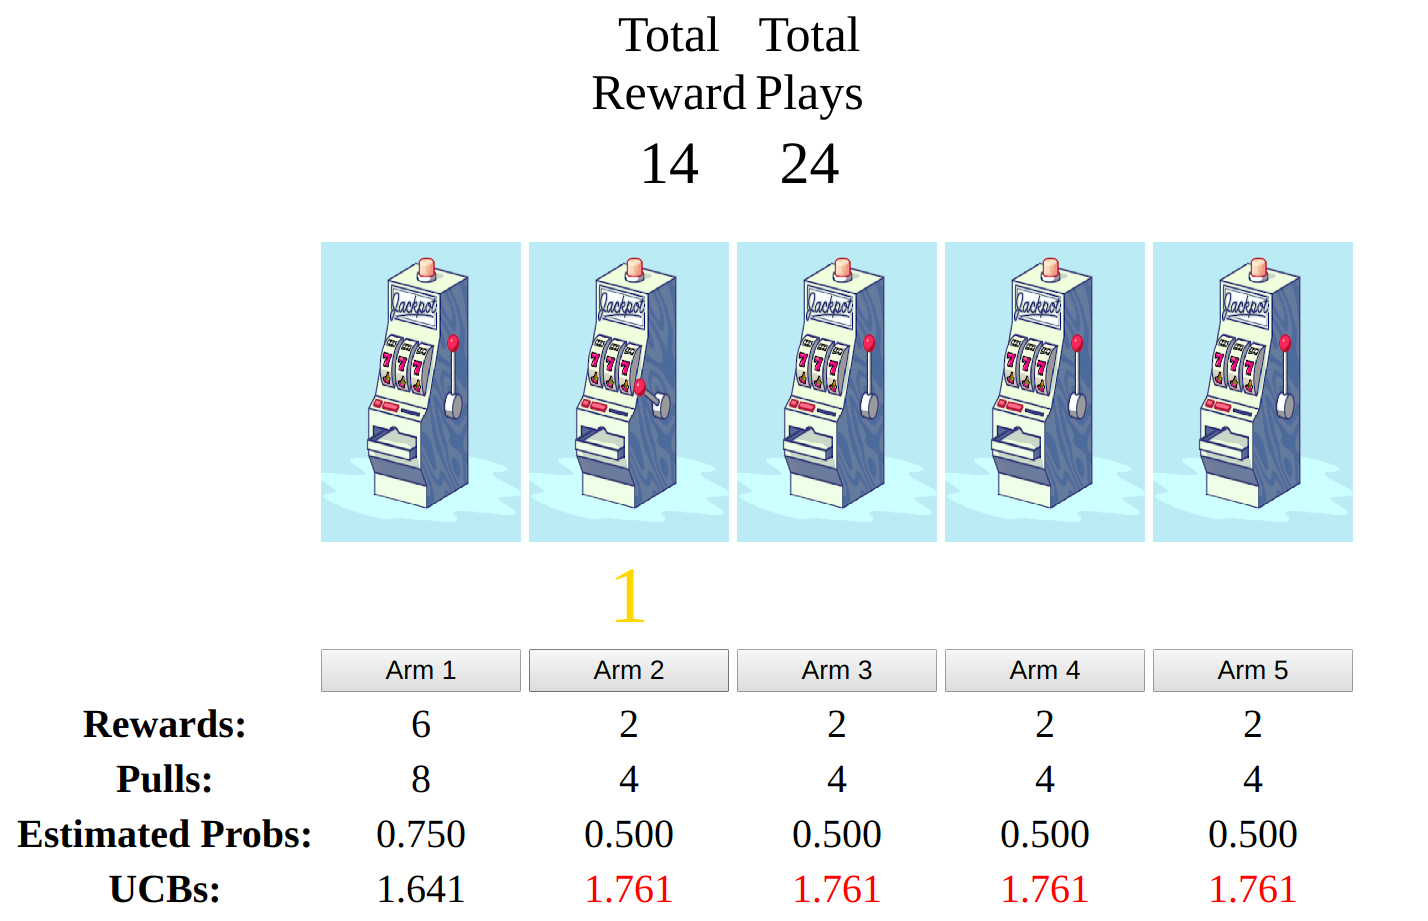
\includegraphics[height=0.55\textheight]{figures/example_of_a_5_arm_bandit_problem.png}
  \end{center}

  \begin{tiny}
  $\hookrightarrow$ Interactive demo
    \href{https://perso.crans.org/besson/phd/MAB_interactive_demo/}{\textcolor{blue}{\texttt{perso.crans.org/besson/phd/MAB\_interactive\_demo/}}}\\
    Ref: [Bandits Algorithms, Lattimore \& Szepesv{\'a}ri, 2019],
    on \href{https://tor-lattimore.com/downloads/book/book.pdf}{\textcolor{blue}{\texttt{tor-lattimore.com/downloads/book/book.pdf}}}
  \end{tiny}

\end{frame}


\subsection{\hfill{}Mathematical model\hfill{}}

\begin{frame}{Mathematical model}

\begin{itemize}
  \item
  Discrete time steps $t = 1, \dots, T$\\
  The \emph{horizon} $T$ is fixed and usually unknown

  \item
  At time $t$, an \emph{agent plays the arm} $A(t)\in\{1,\dots,K\}$,\\
  then she observes the \emph{iid random reward} $r(t) \sim \nu_k$, $r(t)\in\mathbb{R}$

  \pause
  \item
  Usually, we focus on Bernoulli arms $\nu_k = \mathrm{Bernoulli}(\mu_k)$, of mean $\mu_k\in[0,1]$,
  giving binary rewards $r(t) \in\{0,1\}$.

  \pause
  \item
  \textbf{Goal} : maximize the sum of rewards $\sum\limits_{t=1}^T r(t)$

  \item
  or \alert{maximize the sum of expected rewards $\mathbb{E}\left[ \sum\limits_{t=1}^T r(t) \right]$}

  \pause
  \item
  Any efficient policy must balance \alert{between exploration and exploitation}:
  it must explore all arms to discover the best one,
  while exploiting the arms known to be good so far.
\end{itemize}

\end{frame}


\subsection{\hfill{}Naive solutions\hfill{}}

\begin{frame}{Two examples of bad solutions}

  \begin{exampleblock}{$i)$ Pure exploration}
    \begin{itemize}
      \item
      Play arm $A(t) \sim \mathcal{U}(\{1,\dots,K\})$ uniformly at random
      \item
      $\implies$ Mean expected rewards
      $ \frac{1}{T} \mathbb{E}\left[ \sum\limits_{t=1}^T r(t) \right] = \frac{1}{K} \sum\limits_{k=1}^K \mu_k \ll \max_k \mu_k$
    \end{itemize}
  \end{exampleblock}

  \pause

  \begin{exampleblock}{$ii)$ Pure exploitation}
    \begin{itemize}
      \item
        Count the number of samples and the sum of rewards of each arm $N_k(t) = \sum\limits_{s < t} \mathbbm{1}(A(s)=k)$ and $X_k(t) = \sum\limits_{s < t} r(s) \mathbbm{1}(A(s)=k)$
      \item
        Estimate the \alert{unknown} mean $\mu_k$ with $\widehat{\mu_k}(t) = X_k(t) / N_k(t)$
      \item
        Play the arm of maximum empirical mean : $A(t) = \arg\max_k \widehat{\mu_k}(t)$
      \item
        Performance depends on the first draws, and can be very poor!
    \end{itemize}
  \end{exampleblock}

  \begin{tiny}
    $\hookrightarrow$
    Interactive demo
    \href{https://perso.crans.org/besson/phd/MAB_interactive_demo/}{\textcolor{blue}{\texttt{perso.crans.org/besson/phd/MAB\_interactive\_demo/}}}
  \end{tiny}

\end{frame}


\subsection{\hfill{}The \emph{``Upper Confidence Bound''} algorithm\hfill{}}

\begin{frame}{A first solution: \emph{``Upper Confidence Bound''} algorithm}

  \begin{itemize}
    \item
      Compute $\mathrm{UCB}_k(t) = X_k(t) / N_k(t) + \sqrt{\alpha \log(t) / N_k(t)}$ \\
      $=$ an \alert{upper confidence bound} on the \alert{unknown} mean $\mu_k$
    \item
      Play the arm of maximal UCB : $A(t) = \arg\max_k \mathrm{UCB}_k(t)$
      \\
      $\hookrightarrow$ Principle of ``optimism under uncertainty''
    \item
      $\alpha$ balances between \emph{exploitation} ($\alpha\to0$) and \emph{exploration}  ($\alpha\to\infty$)

    \pause

    \item
      \alert{UCB is efficient}:
      the best arm is identified correctly (with high probability) if there are enough samples (for $T$ large enough)
    \item
      $\implies$
      Expected rewards attains the maximum
      ($\forall \alpha>1/2$)
      \[ \text{For~} T\to\infty, \;\;\; \frac{1}{T} \mathbb{E}\left[ \sum\limits_{t=1}^T r(t) \right] \to \max_k \mu_k \]
  \end{itemize}
\end{frame}

\begin{frame}{Elements of the proof for UCB algorithm}

  \begin{block}{Elements of proof of convergence (for $K$ Bernoulli arms)}
    \begin{itemize}[<+->]
      \item
        Suppose the first arm is the best:
        $\textcolor{deeppurple}{\mu^*} = \textcolor{deeppurple}{\mu_1} > \mu_2 \geq \ldots \geq \mu_K$
      \item
        $\mathrm{UCB}_k(t) = X_k(t) / N_k(t) + \sqrt{\alpha \log(t) / N_k(t)}$
      \item
        Hoeffding's inequality gives
        $\mathbb{P}(\mathrm{UCB}_k(t) < \mu_k(t)) \leq \mathcal{O}(\frac{1}{t^{2 \alpha}})$\\
        $\implies$ the different $\mathrm{UCB}_k(t)$ are true ``Upper Confidence Bounds'' on the (unknown) $\mu_k$ (most of the times)
      \item
        And if a suboptimal arm $k>\textcolor{deeppurple}{1}$ is sampled, it implies
        $\mathrm{UCB}_k(t) > \mathrm{UCB}_{\textcolor{deeppurple}{1}}(t)$, but $\mu_k < \textcolor{deeppurple}{\mu_1}$:
        Hoeffding's inequality also proves that any ``wrong ordering'' of the $\mathrm{UCB}_k(t)$ is unlikely
      \item
        We can prove that suboptimal arms $k$ are sampled about $o(T)$ times\\
        $\implies \mathbb{E}\left[ \sum\limits_{t=1}^T r(t) \right] \underset{T\to\infty}{\to} \textcolor{deeppurple}{\mu^*} \times \mathcal{O}(T) + \sum\limits_{k: \Delta_k>0} \mu_k \times o(T)$

        \alert{But\ldots{} at which speed do we have this convergence?}
    \end{itemize}
  \end{block}

\end{frame}


\subsection{\hfill{}Regret of a bandit algorithm\hfill{}}

\begin{frame}{Measure the performance of an algorithm $\mathcal{A}$ with its mean regret $R_{\mathcal{A}}(T)$}

\begin{itemize}
  \item
  Difference in the accumulated rewards between an ``oracle'' and $\mathcal{A}$

  \item
  The ``oracle'' algorithm always plays \textcolor{deeppurple}{the (unknown) best arm $k^* = \arg\max \mu_k$} (we note the best mean \textcolor{deeppurple}{$\mu_{k^*} = \mu^*$})

  \item
  Maximize the sum of expected rewards
  $\Longleftrightarrow$ \alert{minimize the regret}
  %
  \[ \alert{ R_{\mathcal{A}}(T) } = \mathbb{E}\left[ \sum\limits_{t=1}^T \textcolor{deeppurple}{r_{k^*}}(t) \right] - \sum\limits_{t=1}^T \mathbb{E}\left[ r(t) \right] = T \textcolor{deeppurple}{\mu^*} - \sum\limits_{t=1}^T \mathbb{E}\left[ r(t) \right]. \]

\end{itemize}

\pause
\vspace*{10pt}

\begin{exampleblock}{Typical regime for stationary bandits (lower \& upper bounds)}
  \begin{itemize}
  \item
  No algorithm $\mathcal{A}$ can obtain a regret better than
  \hfill{}
  $R_{\mathcal{A}}(T) \geq \Omega(\log(T))$

  \item
  And an efficient algorithm $\mathcal{A}$ obtains
  \hfill{}
  $R_{\mathcal{A}}(T) \leq \mathcal{O}(\log(T))$
  \end{itemize}
\end{exampleblock}

\end{frame}

\subsection{\hfill{}Regret of two UCB algorithms\hfill{}}

\begin{frame}{Regret of the UCB algorithm and another algorithm}

  For any problem with $K$ arms following Bernoulli distributions, of means $\mu_1,\dots,\mu_K \in[0,1]$, and \textcolor{deeppurple}{optimal mean $\mu^*$}, then

  \begin{exampleblock}{For the UCB algorithm}
    \begin{small}
      \[ R_T^{\mathrm{UCB}} \leq ( \sum_{\substack{k=1,\dots,K \\ \mu_k < \textcolor{deeppurple}{\mu^*}}} \frac{8}{(\mu_k - \textcolor{deeppurple}{\mu^*})} ) \log(T) + o(\log(T)) = \mathcal{O}\left( \alert{C(\mu_1,\dots,\mu_K)} \log(T) \right). \]
    \end{small}%
  \end{exampleblock}

  \begin{exampleblock}<2->{For the kl-UCB algorithm: a smaller regret upper-bound}
    \begin{small}
      \[ R_T^{\mathrm{kl}\text{-}\mathrm{UCB}} \leq ( \sum_{\substack{k=1,\dots,K \\ \mu_k < \textcolor{deeppurple}{\mu^*}}} \frac{(\mu_k - \textcolor{deeppurple}{\mu^*})}{\mathrm{kl}(\textcolor{deeppurple}{\mu^*}, \mu_k)} ) \log(T) + o(\log(T)). \]
      %
      If $\mathrm{kl}(x, y) = x \log(x/y) + (1-x) \log((1-x)/(1-y))$ is the binary relative entropy (\emph{ie}, Kullback-Leibler divergence of two Bernoulli of means $x$ and $y$)
    \end{small}%
  \end{exampleblock}

\end{frame}


\section{\hfill{}2. Piece-wise stationary multi-armed bandits problems\hfill{}}

\begin{frame}{2. Piece-wise stationary MAB problems}

  \begin{enumerate}
    \item
    \textcolor{gray}{
      (Stationary) Multi-armed bandits problems
    }
    \vspace*{15pt}

    \item
    \alert{\textbf{%
      Piece-wise stationary multi-armed bandits problems
    }}
    \vspace*{15pt}

    \item
    \textcolor{gray}{
      The B-GLR test and its finite time properties
    }
    \vspace*{15pt}

    \item
    \textcolor{gray}{
      The BGLR-T + klUCB algorithm
    }
    \vspace*{15pt}

    \item
    \textcolor{gray}{
      Regret analysis
    }
    \vspace*{15pt}

    \item
    \textcolor{gray}{
      Numerical simulations
    }
  \end{enumerate}

\end{frame}


\begin{frame}{Non stationary MAB problems}

  \begin{block}{Stationary MAB problems}
    Arm $k$ gives rewards sampled from \textcolor{blue}{the same distribution} for any time step:
    $\forall t, r_k(t) \overset{\text{iid}}{\sim} \nu_k = \mathrm{Bernoulli}(\mu_k)$.
  \end{block}

  \pause
  \begin{alertblock}{Non stationary MAB problems?}
    Arm $k$ gives rewards sampled a \alert{(possibly) different distributions} for any time step:
    $\forall t, r_k(t) \overset{\text{iid}}{\sim} \nu_k\alert{(t)} = \mathrm{Bernoulli}(\mu_k\alert{(t)})$.
  \end{alertblock}

  $\implies$ harder problem!
  And very hard if $\mu_k(t)$ can change at any step!

  \pause
  \begin{block}{\textbf{Piece-wise stationary} problems!}
    $\hookrightarrow$ we focus on the easier case when there are at most $o(\sqrt{T})$ intervals on which the means are all stationary (= \textbf{sequence})
  \end{block}
\end{frame}

\subsection{\hfill{}Definitions\hfill{}}

\begin{frame}{Break-points and stationary sequences}

  Define

  \begin{itemize}
    \item
    The number of break-points\\
    $\Upsilon_T = \sum\limits_{t=1}^{T-1} \mathbbm{1}(\exists k\in \{1,\dots,K\}$ $:$ $\mu_k(t) \neq \mu_k(t+1) )$

    \item
    The $i$-th break-point\\
    $\tau^{i} = \inf\{t > \tau^{i-1} : \exists k : \mu_k(t) \neq \mu_k(t+1)\}$
    \hfill{} (with $\tau^0=0$)
  \end{itemize}

  \begin{block}<2->{\textbf{Hypotheses} on piece-wise stationary problems}
    \begin{itemize}\tightlist
      \item The rewards $r_k(t)$ generated by each arm $k$ are \alert{\emph{iid} on each interval} $[ \tau^{i} + 1, \tau^{i+1} ]$ (the $i$-th sequence)
      \item There are $\Upsilon_T = o(\sqrt{T})$ break-points
      \item And \alert{$\Upsilon_T$ can be known before-hand}
      \item All sequences are ``long enough''
  \end{itemize}
\end{block}
\end{frame}


\begin{frame}[plain]{Example of a piece-wise stationary MAB problem}
  We plots the means \textcolor{red}{$\mu_1(t)$}, \textcolor{green}{$\mu_2(t)$}, \textcolor{blue}{$\mu_3(t)$}
  of $K=3$ arms.
  There are $\Upsilon_T=4$ break-points and $5$ sequences
  between $t=1$ and $t=T=5000$:
  \begin{center}
    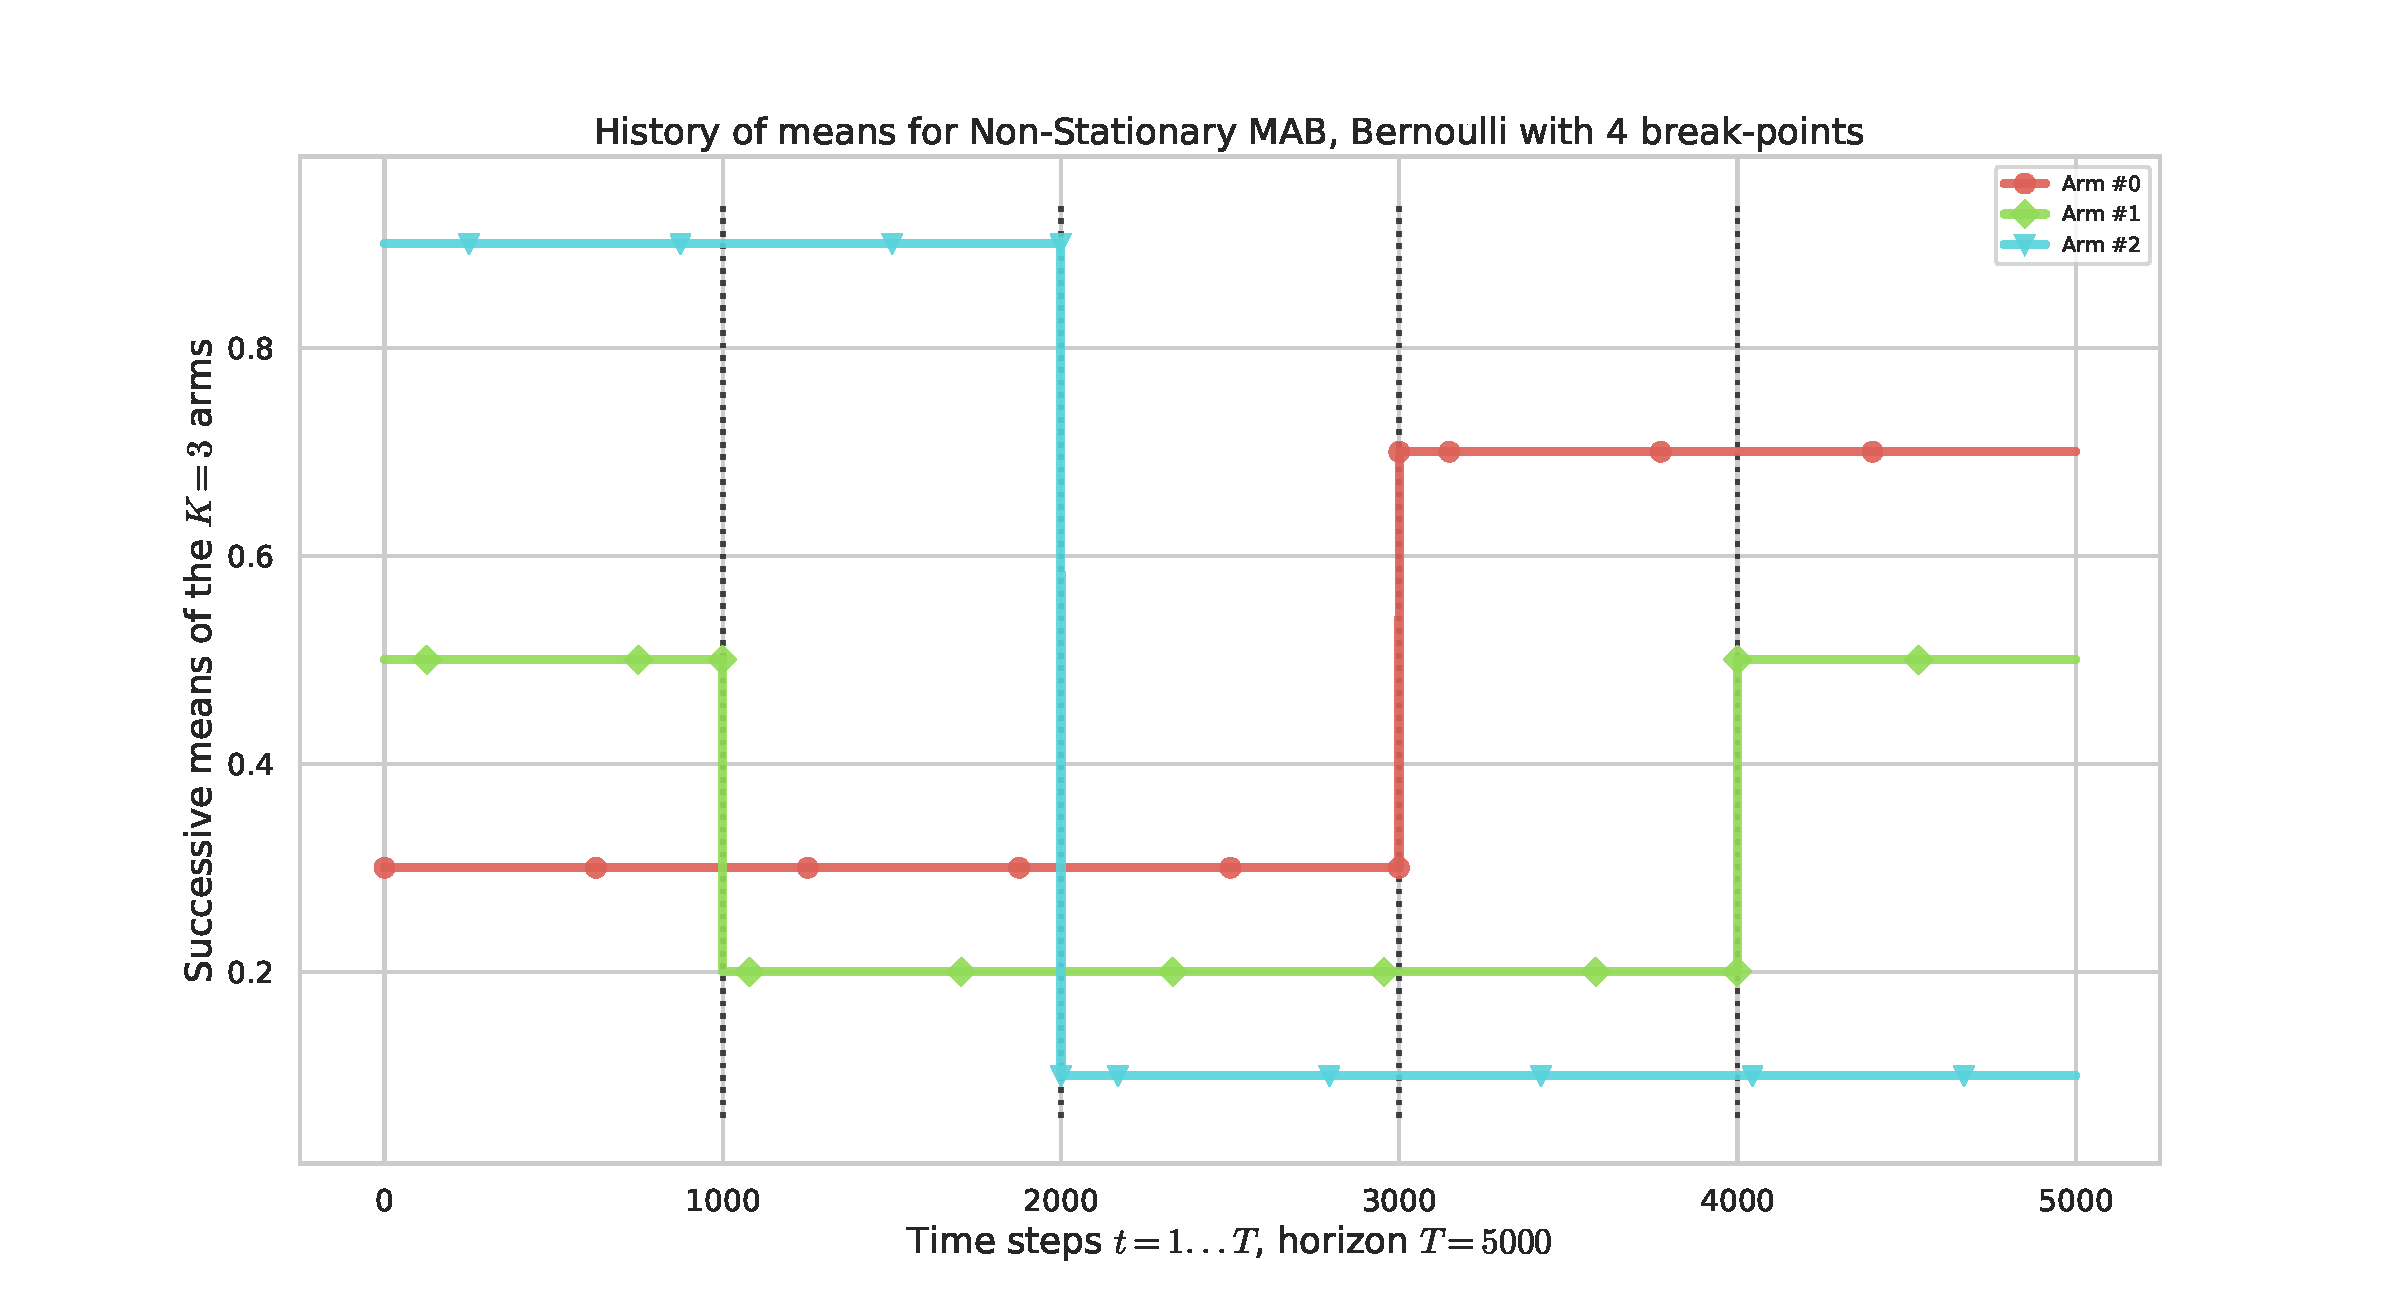
\includegraphics[width=1.00\textwidth]{figures/Problem_1.pdf}
  \end{center}
\end{frame}


\subsection{\hfill{}Extending the definition of regret\hfill{}}

\begin{frame}{Regret for piece-wise stationary bandits?}

  The ``oracle'' algorithm know plays the (unknown) best arm $k^*(t) = \arg\max \mu_k(t)$
  (which changes between stationary sequences)
  %
  \[ \alert{ R_{\mathcal{A}}(T) } = \mathbb{E}\left[ \sum\limits_{t=1}^T r_{k^*(t)}(t) \right] - \sum\limits_{t=1}^T \mathbb{E}\left[ r(t) \right] = \left(\alert{\sum_{t=1}^T \max_k \mu_k(t)} \right) - \sum\limits_{t=1}^T \mathbb{E}\left[ r(t) \right]. \]

\pause
\vspace*{10pt}

\begin{exampleblock}{Typical regime for piece-wise stationary bandits}
  \begin{itemize}
  \item
  The conjectured lower-bound is
  $R_{\mathcal{A}}(T) \geq \Omega(\sqrt{K \Upsilon_T T})$

  \item
  Currently, state-of-the-art algorithms $\mathcal{A}$ obtain
  \[ R_{\mathcal{A}}(T) \leq \mathcal{O}(K \sqrt{\Upsilon_T T \log(T)}) \]
  \end{itemize}
\end{exampleblock}

\end{frame}


\section{\hfill{}3. The B-GLR test and its finite time properties\hfill{}}

\begin{frame}{3. The B-GLR test and its finite time properties}

  \begin{enumerate}
    \item
    \textcolor{gray}{
      (Stationary) Multi-armed bandits problems
    }
    \vspace*{15pt}

    \item
    \textcolor{gray}{
      Piece-wise stationary multi-armed bandits problems
    }
    \vspace*{15pt}

    \item
    \alert{\textbf{%
      The B-GLR test and its finite time properties
    }}
    \vspace*{15pt}

    \item
    \textcolor{gray}{
      The BGLR-T + klUCB algorithm
    }
    \vspace*{15pt}

    \item
    \textcolor{gray}{
      Regret analysis
    }
    \vspace*{15pt}

    \item
    \textcolor{gray}{
      Numerical simulations
    }
  \end{enumerate}

\end{frame}


\subsection{\hfill{}Break-point detection\hfill{}}

\begin{frame}{The break-point detection problem}

  Imagine the following game\ldots

  \begin{itemize}
    \item You observe data $X_1,X_2,\ldots,X_t,\ldots \in[0,1]$
    \item You know $X_t$ is generated by a certain (unknown) distribution

    \item \alert{Your goal} is to distinguish between two hypotheses:
    \begin{itemize}
      \item[\textcolor{deeppurple}{$\mathcal{H}_0$}] \textcolor{deeppurple}{The distributions have the same mean \hfill{} (``no break-point'')\\
      $\exists \mu_0, \mathbb{E}[X_1] = \mathbb{E}[X_2] = \ldots = \mathbb{E}[X_t] = \mu_0$}

      \item[\textcolor{meca}{$\mathcal{H}_1$}] \textcolor{meca}{The distributions have changed mean at a break-point at time $\tau$ \\
      $\exists \mu_0, \mu_1, \tau, \mathbb{E}[X_1] = \ldots = \mathbb{E}[X_{\tau}] = \mu_0, \mathbb{E}[X_{\tau+1}] = \mathbb{E}[X_{\tau+2}] = \ldots = \mu_1$}
      % $\exists \mu_0, \mu_1, \exists \tau, \forall t \leq \tau, \mathbb{E}[X_t] = \mu_0 \text{ and } \forall t \geq \tau + 1, \mathbb{E}[X_t] = \mu_1$
    \end{itemize}
  \end{itemize}

  \pause
  A \alert{sequential break-point detection} is a stopping time,
  measurable under $\mathcal{F}_t = \sigma(X_1,\dots,X_t)$,
  which rejects the hypothesis \textcolor{deeppurple}{$\mathcal{H}_0$}
  when $\widehat{\tau} < +\infty$.

\end{frame}


\subsection{\hfill{}Likelihood ratio test for Bernoulli observations\hfill{}}

\begin{frame}{Bernoulli likelihood ratio test}

  \textbf{Hypothesis}: all distributions are Bernoulli

  The problem boils down to distinguishing
  \begin{itemize}
    \item[\textcolor{deeppurple}{$\mathcal{H}_0$}:]
    \textcolor{deeppurple}{$(\exists \mu_0 : \forall i\in\mathbb{N}^*, X_i \overset{\text{i.i.d.}}{\sim} \cB(\mu_0))$},
    against the alternative
    \item[\textcolor{meca}{$\mathcal{H}_1$}:]
    \textcolor{meca}{$(\exists \mu_0 \neq \mu_1, \tau > 1 : X_1, \ldots, X_\tau \overset{\text{i.i.d.}}{\sim} \cB(\mu_0) \text{~et~} X_{\tau+1}, \ldots \overset{\text{i.i.d.}}{\sim} \cB(\mu_1))$}.
  \end{itemize}

  \pause

  The \alert{Likelihood Ratio statistic} for this hypothesis test, after observing $X_1,\dots,X_n$, is given by
  \[ \mathcal{L}(n) = \frac{\sup\limits_{\textcolor{meca}{\mu_0,\mu_1,\tau < n}}\ell(X_1,\dots,X_n ; \textcolor{meca}{\mu_0,\mu_1,\tau})}{\sup\limits_{\textcolor{deeppurple}{\mu_0}}\ell(X_1,\dots,X_n ;\textcolor{deeppurple}{\mu_0})},\]
  %
  where $\ell(X_1,\dots,X_n ; \textcolor{deeppurple}{\mu_0})$ (resp. $\ell(X_1,\dots,X_n ; \textcolor{meca}{\mu_0,\mu_1,\tau})$) is the likelihood of the observations under a model in \textcolor{deeppurple}{$\mathcal{H}_0$} (resp. \textcolor{meca}{$\mathcal{H}_1$}).

  \pause

  \alert{$\hookrightarrow$ High values of this statistic tends to reject \textcolor{deeppurple}{$\mathcal{H}_0$} over \textcolor{meca}{$\mathcal{H}_1$}.}

\end{frame}

\begin{frame}{Expression of the Bernoulli Likelihood ratio}

  We can rewrite this statistic
  $\mathcal{L}(n) = \frac{\sup\limits_{\textcolor{meca}{\mu_0,\mu_1,\tau < n}}\ell(X_1,\dots,X_n ; \textcolor{meca}{\mu_0,\mu_1,\tau})}{\sup\limits_{\textcolor{deeppurple}{\mu_0}}\ell(X_1,\dots,X_n ;\textcolor{deeppurple}{\mu_0})}$,
  by using Bernoulli likelihood, and shifting means $\widehat{\mu}_{k:k'} = \frac{1}{k'-k+1} \sum\limits_{s=k}^{k'} X_s$ :

  \begin{align*}
    \log \mathcal{L}(n) = \sup_{s \in \{2,\dots,n-1\}} \bigl[
      & s \times \mathrm{kl} (\underbrace{\widehat{\mu}_{1:s}}_{\text{before change}},\underbrace{\widehat{\mu}_{1:n}}_{\text{all data}} ) \\
      + & (n-s) \times \mathrm{kl} (\underbrace{\widehat{\mu}_{s+1:n}}_{\text{after change}},\underbrace{\widehat{\mu}_{1:n}}_{\text{all data}} ) \bigr].
  \end{align*}

  \begin{footnotesize}
    Where $\mathrm{kl}(x,y) =x \ln\bigl(x/y\bigr) + (1-x)\ln\bigl((1-x)/(1-y)\bigr)$ is the binary relative entropy
  \end{footnotesize}

\end{frame}


\subsection{\hfill{}The BGLR-T\hfill{}}

\begin{frame}{The Bernoulli Generalized likelihood ratio test (BGLR)}

  \begin{itemize}
    \item
    We can extend the Bernoulli likelihood ratio test if the observations are \alert{sub-Bernoulli}.
    \item
    And any bounded distributions on $[0,1]$ is sub-Bernoulli
    \item
    $\implies$ the BGLR test can be applied for any bounded observations!
  \end{itemize}

  % \begin{block}{Sub-Bernoulli distributions}
  %   If $\nu$ is supported in $[0,1]$,
  %   $\nu$ is \emph{sub-Bernoulli} if it verifies
  %   $\mathbb{E}_{X\sim\nu}\left[e^{\lambda X}\right] \leq  1-\mu + \mu e^\lambda = \mathbb{E}_{X\sim \mathrm{Bernoulli}(\mu)} [e^{\lambda X}]$.
  %   % where $\cB(\mu)$ est la loi de Bernoulli de moyenne $\mu$.
  % \end{block}

  \pause

  \begin{block}{The BGRL-T sequential break-point detection test}
    The \alert{BGLR-T} is the stopping time
    \begin{small}
    \[ \widehat{\tau}_{\delta} = \inf \bigl\{ n \in \mathbb{N}^* : \max_{s \in \{2,\dots,n-1\}} \bigl[s \, \mathrm{kl}\left(\widehat{\mu}_{1:s},\widehat{\mu}_{1:n}\right) + (n-s) \, \mathrm{kl}\left(\widehat{\mu}_{s+1:n},\widehat{\mu}_{1:n}\right)\bigr] \geq \beta(n,\delta) \bigr\} \]
    \end{small}
    with a \alert{threshold function} $\beta(n,\delta)$ specified later.
  \end{block}

\end{frame}


\subsection{\hfill{}False alarm\hfill{}}

\begin{frame}{Probability of false alarm}

  A good test should not detect any break-point if there is no break-point to detect\ldots

  \begin{block}{False alarm}
    The stopping time is $\widehat{\tau}_\delta$,
    and a break-point is detected if $\widehat{\tau}_\delta < \infty$.

    Let $\mathbb{P}_{\textcolor{deeppurple}{\mu_0}}$ be a probability model under which the observations are $X_t \in[0,1]$
    and \textcolor{deeppurple}{$\mathbb{E}[X_t] = \mu_0$ for all $t$}.

    The \alert{false alarm probability} is $\mathbb{P}_{\textcolor{deeppurple}{\mu_0}}(\widehat{\tau}_\delta < \infty)$.
  \end{block}

  \alert{$\implies$ Goal: controlling the false alarm event!} (in high probability)

\end{frame}

\begin{frame}{First result for the BGLR test}

  \begin{block}{Controlling the false alarm probability}
    For any \alert{confidence level} $0<\delta<1$,
    the BGLR test satisfies
    \[ \mathbb{P}_{\textcolor{deeppurple}{\mu_0}}(\widehat{\tau}_\delta < \infty) \leq \delta \]
    with the threshold function
    \[ \beta(n,\delta)= 2\,\mathcal{T}\left(\frac{\ln(3n\sqrt{n}/\delta)}{2}\right) + 6\ln(1+\ln(n)) \simeq \ln(3n \sqrt{n}/\delta).\]
  \end{block}

  Where $\mathcal{T}(x)$ verifies $\mathcal{T}(x)\simeq x + \ln(x)$ for $x$ large enough

  \begin{exampleblock}<2>{Proof ?}
    Hard to explain in a short time\ldots\\
    %  we used time-uniform concentration inequalities
    $\hookrightarrow$ pre-print on
    \href{https://hal.inria.fr/hal-02006471}{\textcolor{blue}{HAL-02006471}}
    and
    \href{https://arxiv.org/abs/1902.01575}{\textcolor{blue}{arXiv:1902.01575}}
  \end{exampleblock}

\end{frame}

\subsection{\hfill{}Delay of detection\hfill{}}

\begin{frame}{Delay of detection}

  A good test should detect a break-point ``fast enough'' if there is a break-point to detect, with enough samples before the break-point

  \begin{block}{Delay of detection}
    Let $\mathbb{P}_{\textcolor{meca}{\mu_0,\mu_1,\tau}}$ be a probability model under which $X_t \in[0,1]$ and \textcolor{meca}{$X_t$ a mean $\mu_0$ for all $t \leq \tau$, and $\mu_1$ for all $t > \tau$,
    with $\mu_0 \neq \mu_1$}.

    The \alert{gap} of this break-point is $\Delta = |\mu_0 - \mu_1|$.

    The \alert{delay of detection} is $u = \widehat{\tau}_{\delta} - \tau$.
  \end{block}

  \alert{$\implies$ Goal: controlling the delay of detection!} (in high probability)

\end{frame}

\begin{frame}{Second result for the BGLR test}

  \begin{block}{Controlling the delay of detection}
      On a break-point of amplitude $\Delta = |\mu_1 - \mu_0|$,
      the B-GLRT test satisfies
      \begin{small}
      \[ \mathbb{P}_{\textcolor{meca}{\mu_0,\mu_1,\tau}} (\widehat{\tau}_{\delta} \geq \textcolor{meca}{\tau} + u) \leq \exp\left( -\frac{2\textcolor{meca}{\tau} u}{\textcolor{meca}{\tau} + u}\left(\max\left[ 0, \Delta - \sqrt{\frac{\textcolor{meca}{\tau} + u}{2\textcolor{meca}{\tau} u} \beta(\textcolor{meca}{\tau} + u,\delta)} \right]\right)^2 \right). \]
      \end{small}
      with the same threshold function
      $\beta(n,\delta) \simeq \ln(3n \sqrt{n}/\delta)$.
  \end{block}

  \begin{exampleblock}{Consequence}
    In high probability, the delay $\widehat{\tau}_\delta$ of BGLR is $\mathcal{O}(\Delta^{-2} \ln(1/\delta))$ if enough samples are observed before the break-point at time $\tau$.
    % (at least) $\Delta^{-2} \ln(1/\delta)$ samples, the detection delay of BGLR has the same magnitude.
  \end{exampleblock}

\end{frame}


\subsection{\hfill{}Summary of results for BGLR-T\hfill{}}

\begin{frame}{BGLR is an efficient break-point detection test!}

  \begin{itemize}
    \item
    We just saw that by choosing
    \begin{itemize}\tightlist
      \item
      a confidence level $\delta$,
      \item
      and a good threshold function $\beta(n,\delta) \simeq \ln(3n^{3/2}/\delta)$
    \end{itemize}
    \item
    we can control the two properties of the BGLR test:
    \begin{itemize}\tightlist
      \item
        its \alert{false alarm probability}:
        $\mathbb{P}_{\textcolor{darkpurple}{\mu_0}}(\widehat{\tau}_\delta < \infty) \leq \delta$
      \item
        its \alert{detection delay}:
        $\mathbb{P}_{\textcolor{meca}{\mu_0,\mu_1,\tau}} (\widehat{\tau}_{\delta} \geq \tau + u)$ decreases exponentially fast wrt $u$
      (if there are enough samples before and after the break-point).
    \end{itemize}

    \item
    $\implies$ it is an efficient break-point detection test
  \end{itemize}

  \pause
  \begin{block}{Finite time guarantees}
    The two guarantees are \alert{finite time} and not asymptotic, this kind of results are quite recent!
    %
    \hfill{}
    {\tiny
      \textcolor{gray}{[Maillard, ALT, 2019]}
      \textcolor{gray}{[Lai \& Xing, Sequential Analysis, 2010]}
    }
  \end{block}

\end{frame}

\section{\hfill{}4. The BGLR-T + klUCB algorithm\hfill{}}

\begin{frame}{4. The BGLR-T + klUCB algorithm}

  \begin{enumerate}
    \item
    \textcolor{gray}{
      (Stationary) Multi-armed bandits problems
    }
    \vspace*{15pt}

    \item
    \textcolor{gray}{
      Piece-wise stationary multi-armed bandits problems
    }
    \vspace*{15pt}

    \item
    \textcolor{gray}{
      The B-GLR test and its finite time properties
    }
    \vspace*{15pt}

    \item
    \alert{\textbf{%
      The BGLR-T + klUCB algorithm
    }}
    \vspace*{15pt}

    \item
    \textcolor{gray}{
      Regret analysis
    }
    \vspace*{15pt}

    \item
    \textcolor{gray}{
      Numerical simulations
    }
  \end{enumerate}

\end{frame}

\subsection{\hfill{}BGRL test + kl-UCB index\hfill{}}

\begin{frame}{Our algorithm: BGRL test + kl-UCB index (1/2)}

  % TODO expliquer kl-UCB
  % TODO expliquer réinitialisation mémoire
  % TODO expliquer comment utiliser le test
  % TODO expliquer local/global

  \begin{block}{Main ideas}
    \begin{itemize}
      % \item Forced uniform random exploration with probability $\alpha$
      \item We compute a UCB index on each arm
        % $\mbox{kl-UCB}_k(t)$
      \item Most of the times, we select the arm with highest index
      $A_t = \arg\max\limits_{k\in \{1,\dots,K\}} \mbox{kl-UCB}_k(t)$
      \item We use a BGLR test to detect changes on the played arm
      \item If a break-point is detected, we reset the memories of \emph{all arms}
    \end{itemize}
  \end{block}

  \pause

  \begin{exampleblock}{The kl-UCB indexes}
    \begin{itemize}
      \item $\tau_k(t)$ is the time of last restart of arm $k$ before time $t$,
      \item $n_k(t)$ counts the the selections, and $\widehat{\mu}_k(t)$ is the empirical means of observations since the last restart of arm $k$,
      % = \sum\limits_{s=\tau_k(t)+1}^{t} \mathbbm{1}(A_s=k)$
      % la moyenne empirique des récompenses obtenues entre la dernière réinitialisation et l'instant $t$.
      %= (\sum_{s=\tau_i(t)+1}^{t}X_{i,s} \mathbbm{1}(A_s=i))/n_i(t)$ (si $n_i(t)\neq0$)
      \item Let {\small $\mbox{kl-UCB}_k(t) = \max \bigl\{ q\in[0,1] : n_k(t) \times \mathrm{kl}\left(\widehat{\mu}_k(t),q\right) \leq f(t - \tau_k(t)) \bigr\}$ }
      \item $f(t) = \ln(t) + 3 \ln(\ln(t))$ controls the width of the UCB.
    \end{itemize}
  \end{exampleblock}

\end{frame}

\begin{frame}{Our algorithm: BGRL test + kl-UCB index (2/2)}

  % % \GLRklUCB{} repose sur le calcul d'un \emph{indice} (de type \mathrm{kl}UCB{} \cite{KLUCBJournal}) pour chaque bras,  et choisit en général le bras d'indice le plus élevé.
  % Soit $\tau_i(t)$ l'instant de la dernière réinitialisation pour le bras $i$ avant le temps $t$, $n_i(t) = \sum_{s=\tau_i(t)+1}^{t} \mathbbm{1}(A_s=i)$ le nombre de sélections et $\widehat{\mu}_i(t)$
  % %= (\sum_{s=\tau_i(t)+1}^{t}X_{i,s} \mathbbm{1}(A_s=i))/n_i(t)$ (si $n_i(t)\neq0$)
  % la moyenne empirique des récompenses obtenues entre la dernière réinitialisation et l'instant $t$.

  % % L'indice du bras $i$ à l'instant $t$ est défini par
  % % $\UCB_i(t) = \max \bigl\{ q\in[0,1] : n_i(t) \times \mathrm{kl}\left(\widehat{\mu}_i(t),q\right) \leq f(t - \tau_i(t)) \bigr\}$ (l. $6$) avec la fonction d'exploration $f(t) = \ln(t) + 3 \ln(\ln(t))$.
  % % La détection d'une rupture sur le bras qui vient d'être joué
  % % produit une réinitialisation (l. $12$),

  \begin{exampleblock}{How do we use the BGLR test? \hfill{} (parameter $\delta$)}
    From observations $Z_1,\cdots,Z_n$
    % $\mbox{BGLRT}_\delta(Z_1,\dots,Z_n) = \mathrm{True}$
    we detect a break-point
    with confidence level $\delta$
    when
    % \begin{footnotesize}
      \[
        \sup_{1 < s < n} \left[s \times \mathrm{kl} \left( \widehat{Z}_{1:s}, \widehat{Z}_{1:n}\right) + (n-s) \times \mathrm{kl} \left( \widehat{Z}_{s+1:n}, \widehat{Z}_{1:n} \right) \right] \geq \beta(n,\delta)
        \]
    % \end{footnotesize}%
    % We use $\beta(n,\delta) \simeq \ln(3n^{3/2}/\delta)$
  \end{exampleblock}

  \pause

  \begin{exampleblock}{Forced exploration \hfill{} (parameter $\alpha$)}
    \begin{itemize}
      \item We use a forced exploration uniformly on all arms\ldots\\
        \emph{ie}, in average, arm $k$ is forced to be sampled at least $T \times \alpha / K$ times
      \item $\implies$ so we can detect break-points on all the arms
      \item and not only on the arm played by the kl-UCB indexes
      % (lignes $5$-$6$), qui assure que chaque bras est suffisamment échantillonné, afin que les ruptures puissent aussi être détectées sur les bras actuellement sous-échantillonnés par l'algorithme de bandit.
    \end{itemize}
  \end{exampleblock}

\end{frame}

\begin{frame}{The BGLR + kl-UCB algorithm}

\begin{columns}
\begin{column}{0.1\textwidth}
  %
\end{column}
\begin{column}{0.9\textwidth}  %%<--- here

\begin{footnotesize}
  % Documentation at http://mirror.ctan.org/tex-archive/macros/latex/contrib/algorithm2e/doc/algorithm2e.pdf if needed
  % Or https://en.wikibooks.org/wiki/LaTeX/Algorithms#Typesetting_using_the_algorithm2e_package
  \removelatexerror% Nullify \@latex@error % Cf. http://tex.stackexchange.com/a/82272/
  \begin{algorithm}[H]
      % XXX Options
      % \LinesNumbered  % XXX Option to number the line
      % \RestyleAlgo{boxed}
      % XXX Input, data and output
      \Donnees{\emph{Parameters of the problem} : $T\in\mathbb{N}^*$, $K\in\mathbb{N}^*$\;}
      \Donnees{\emph{Parameters of the algorithm} : $\alpha \in (0, 1)$, $\delta>0$\;}
      % \Donnees{\emph{Option} : redémarrages \textbf{Locaux} ou \textbf{Globaux}\;}
      % \KwData{Data}
      % \KwResult{Result}
      % XXX Algorithm
      \textbf{Initialisation : } $\forall k \in \{1,\dots,K\}$, $\tau_k = 0$ and $n_k = 0$ \\
      \For{$t=1,2,\ldots, T$}{
          \pause
          \uIf{
              $t \mod \left\lfloor \frac{K}{\alpha}\right\rfloor \in \{1,\dots,K\}$
          }{
              $A_t = t \mod \left\lfloor \frac{K}{\alpha}\right\rfloor$
              \tcp*[f]{forced exploration} \\
          }
          \Else{
              $A_t = \arg\max\limits_{k\in \{1,\dots,K\}} \mbox{kl-UCB}_k(t)$
              % \tcp*[f]{avec les indices}
              % comme défini en \eqref{def:UCB}
          }
          \pause
          \mbox{Play arm} $k=A_t$, and update play count $n_{A_t} = n_{A_t} + 1$ \\
          \mbox{Observe a reward} $X_{A_t,t}$ : $Z_{A_t, n_{A_t}} = X_{A_t,t}$ \\
          \pause
          \uIf{
              $\mathrm{BGLRT}_\delta(Z_{A_t,1}, \cdots, Z_{A_t, n_{A_t}})$ = True
          }
          {
              % \uSi{Redémarrages \textbf{globaux}}{
                  $\forall k, \tau_k = t$ and $n_k = 0 $.\tcp*[f]{reinitialize}
                  % \tcp*[f]{redémarrages globaux}
                  % }
              % \Sinon{
                  % $\tau_{A_t} = t$ and $n_{A_t} = 0$
                  % \tcp*[f]{redémarrage local}
              % }
          }
      }
  \end{algorithm}
\end{footnotesize}

\end{column}
\end{columns}

\end{frame}


\section{\hfill{}5. Regret analysis\hfill{}}

\begin{frame}{5. Regret analysis}

  \begin{enumerate}
    \item
    \textcolor{gray}{
      (Stationary) Multi-armed bandits problems
    }
    \vspace*{15pt}

    \item
    \textcolor{gray}{
      Piece-wise stationary multi-armed bandits problems
    }
    \vspace*{15pt}

    \item
    \textcolor{gray}{
      The B-GLR test and its finite time properties
    }
    \vspace*{15pt}

    \item
    \textcolor{gray}{
      The BGLR-T + klUCB algorithm
    }
    \vspace*{15pt}

    \item
    \alert{\textbf{%
      Regret analysis
    }}
    \vspace*{15pt}

    \item
    \textcolor{gray}{
      Numerical simulations
    }
  \end{enumerate}

\end{frame}

\subsection{\hfill{}Hypotheses\hfill{}}

\begin{frame}{Hypotheses of our theoretical analysis}

  \begin{itemize}
    \item
    Denote $\tau^{i}$ the position of $i$-th break-point
    \item
    and $\mu_k^{i}$ the mean of arm $k$ on segment $[\tau^i, \tau^{i+1}]$.
    \item
    Let $b(i) \in \arg\max_k \mu_k^{i} $
    \item
    and the largest gap at break-point $i$ is
    $\Delta^{i} = \max\limits_{k=1,\dots,K} |\mu_k^{i} - \mu_k^{i-1}| >0$.
  \end{itemize}

  \pause
  \begin{block}{Assumption}
    Let $d^{i} = d^{i}(\alpha,\delta) = \lceil \frac{4K}{\alpha(\Delta^{i})^2}\beta(T,\delta) + \frac{K}{\alpha} \rceil$.

    Assume that all sequences are long enough:
    \[ \forall i \in \{1,\dots,\Upsilon_T\}, \;\;\;\; \tau^{i} - \tau^{i-1} \geq 2\max( d^{i}, d^{i-1} ). \]
  \end{block}

  The minimum length of the $i$-th sequence depends on the amplitude of the changes at \textcolor{darkred}{the beginning} and \textcolor{darkblue}{the end} of the sequence (\textcolor{darkred}{$\Delta^i$} and \textcolor{darkblue}{$\Delta^{i+1}$})

\end{frame}


\subsection{\hfill{}Regret upper-bound\hfill{}}

\begin{frame}{Theoretical result}

  Under this hypothesis, we obtained a \emph{finite time}
  upper-bound on the regret $R_T$,
  with explicit dependency from the problem difficulty.

  The exact bound uses:
  \begin{itemize}
    \item
    the divergences $\mathrm{kl}(\mu_{k}^{i},\mu_{b(i)}^{i})$ to account for the difficulty of the stationary problem on any sequence,
    \item
    $\Delta^{i}$ express the difficulty of detecting the $i$-th break-point,
  \end{itemize}
  as well as
  \begin{itemize}
    \item
    the parameter $\alpha$ probability of forced exploration,
    \item
    and the parameter $\delta$ the confidence level of the break-point detection algorithm.
  \end{itemize}

\end{frame}


\begin{frame}{Simplified form of the regret upper-bound}

  \begin{block}{Regret upper bound for BGLR + kl-UCB}
    \begin{itemize}
      \item
      Let $\alpha = \sqrt{\Upsilon_T \ln(T) / T}$ and $\delta = 1 / \sqrt{\Upsilon_T T}$
      \item
      And for a problem satisfying our assumption
      \pause
      \item
      Then the regret of our algorithm, with parameters $\alpha$ and $\delta$, satisfies
      %
      \[ R_T =\mathcal{O}\left( \frac{K}{\left(\textcolor{deeppurple}{\Delta^{\text{change}}}\right)^2}\sqrt{T \Upsilon_T \ln(T)} + \frac{(K-1)}{\textcolor{meca}{\Delta^{\text{opt}}}} \Upsilon_T\ln(T) \right),\]
      \item
      with $\textcolor{deeppurple}{\Delta^{\text{change}}} = \min_{i} \Delta^{i}$ \textcolor{deeppurple}{the smallest detection gap between two stationary segments},
      \item
      $\textcolor{meca}{\Delta^{\text{opt}}}$
      \textcolor{meca}{the smallest value of sub-optimality gap on a stationary segment}.
      % ($\min_{k: \mu_k(t) < \mu_{k^*(t)}(t)} \mu_{k^*(t)}(t) - \mu_k(t)$)
    \end{itemize}
  \end{block}

\pause
$\implies$ $R_T = \mathcal{O}(K \sqrt{T \Upsilon_T \log(T)})$ if we hide the dependency on the gaps.

\end{frame}


\subsection{\hfill{}Comparison with other algorithms\hfill{}}

\begin{frame}{Comparison with other state-of-the-art approaches}

  \begin{exampleblock}{Our algorithm (BGLR + kl-UCB)}
    \begin{itemize}
      \item Hypotheses: bounded rewards, known $T$ and $\Upsilon_T = o(\sqrt{T})$, and long enough stationary sequences
      \item We obtain $R_T = \mathcal{O}(K \sqrt{\Upsilon_T T \log(T)})$
    \end{itemize}
  \end{exampleblock}

  \pause
  And two recent competitors:

  % \begin{block}{Exp3.S \hfill{} \textcolor{gray}{[Auer et al, 2002]}}
  %   \begin{itemize}
  %     \item Hypotheses: just bounded rewards
  %     \item $R_T = \mathcal{O}(K \sqrt{\Upsilon_T T})$
  %     \item But usually poor in practice
  %   \end{itemize}
  % \end{block}

  \begin{block}{CUSUM-UCB \hfill{} \textcolor{gray}{[Liu \& Lee \& Shroff, AAAI 2018]}}
    \begin{itemize}
      \item Also require \alert{prior knowledge of a lower-bound on the gaps}
      \item They obtained $R_T = \mathcal{O}(K \sqrt{\Upsilon_T T \log(T / \Upsilon_T)})$
    \end{itemize}
  \end{block}

  \begin{block}{M-UCB \hfill{} \textcolor{gray}{[Cao \& Zhen \& Kveton \& Xie, AISTATS 2019]}}
    \begin{itemize}
      \item Also require \alert{prior knowledge of a lower-bound on the gaps}
      \item They obtained $R_T = \mathcal{O}(K \sqrt{\Upsilon_T T \log(T)})$
    \end{itemize}
  \end{block}

\end{frame}


\section{\hfill{}6. Numerical simulations\hfill{}}

\begin{frame}{6. Numerical simulations}

  \begin{enumerate}
    \item
    \textcolor{gray}{
      (Stationary) Multi-armed bandits problems
    }
    \vspace*{15pt}

    \item
    \textcolor{gray}{
      Piece-wise stationary multi-armed bandits problems
    }
    \vspace*{15pt}

    \item
    \textcolor{gray}{
      The B-GLR test and its finite time properties
    }
    \vspace*{15pt}

    \item
    \textcolor{gray}{
      The BGLR-T + klUCB algorithm
    }
    \vspace*{15pt}

    \item
    \textcolor{gray}{
      Regret analysis
    }
    \vspace*{15pt}

    \item
    \alert{\textbf{%
      Numerical simulations
    }}
  \end{enumerate}

\end{frame}


\subsection{\hfill{}Setup of the experiments\hfill{}}

\begin{frame}{Numerical simulations}

  \begin{block}{We consider three problems with}
    \begin{itemize}
      \item
      $K=3$ arms, Bernoulli distributed
      \item
      $T=5000$ time steps (fixed horizon)
      \item
      $\Upsilon_T=4$ break-points ($=5$ stationary sequences)
      \item
      Algorithms can use this prior knowledge of $T$ and $\Upsilon_T$
      \item
      $1000$ independent runs, we plot the average regret
    \end{itemize}
  \end{block}

  \pause

  \begin{exampleblock}{Reference}
    \begin{itemize}
      \item
      We used my open-source Python library for simulations of multi-armed bandits problems, \textbf{SMPyBandits}\\
      $\hookrightarrow$ Published online at \href{https://SMPyBandits.GitHub.io}{\textcolor{blue}{\texttt{SMPyBandits.GitHub.io}}}
      \item
      More experiments are included in the long version of the paper!\\
      $\hookrightarrow$ pre-print on
      \href{https://hal.inria.fr/hal-02006471}{\textcolor{blue}{HAL-02006471}}
      and
      \href{https://arxiv.org/abs/1902.01575}{\textcolor{blue}{arXiv:1902.01575}}
    \end{itemize}
  \end{exampleblock}

\end{frame}


\begin{frame}[plain]{Problem 1: only local changes}
  \begin{center}
    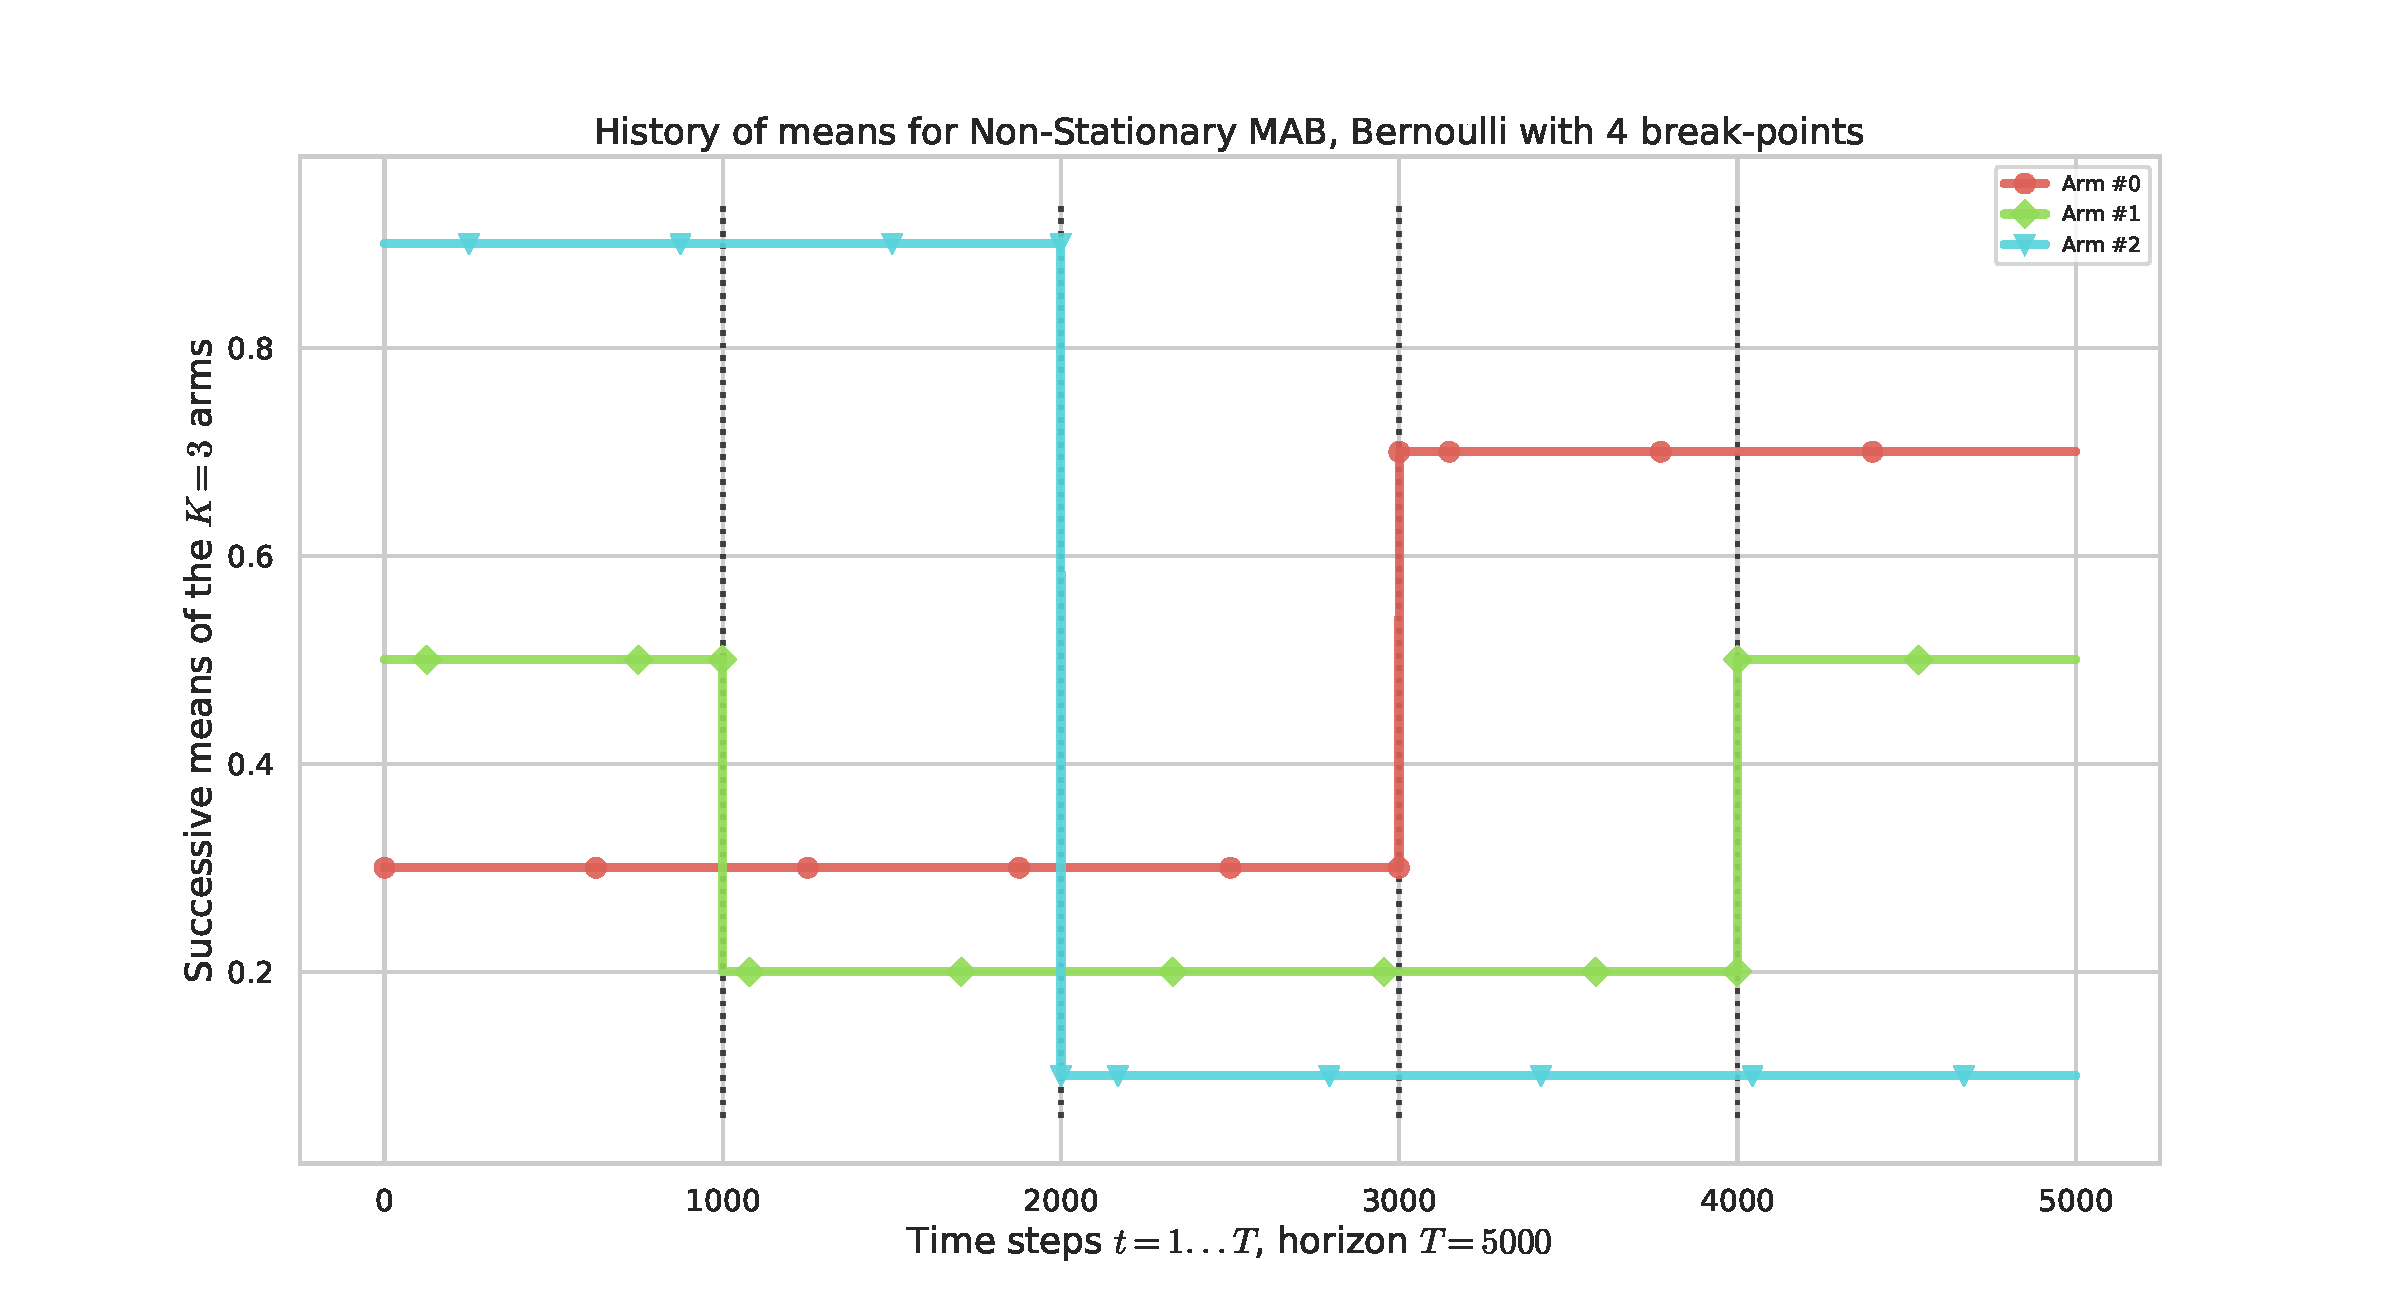
\includegraphics[width=1.00\textwidth]{figures/Problem_1.pdf}
  \end{center}
  We plots the means:
  \textcolor{red}{$\mu_1(t)$},
  \textcolor{green}{$\mu_2(t)$},
  \textcolor{blue}{$\mu_3(t)$}.
\end{frame}

\begin{frame}[plain]{Results on problem 1}
  \centering
  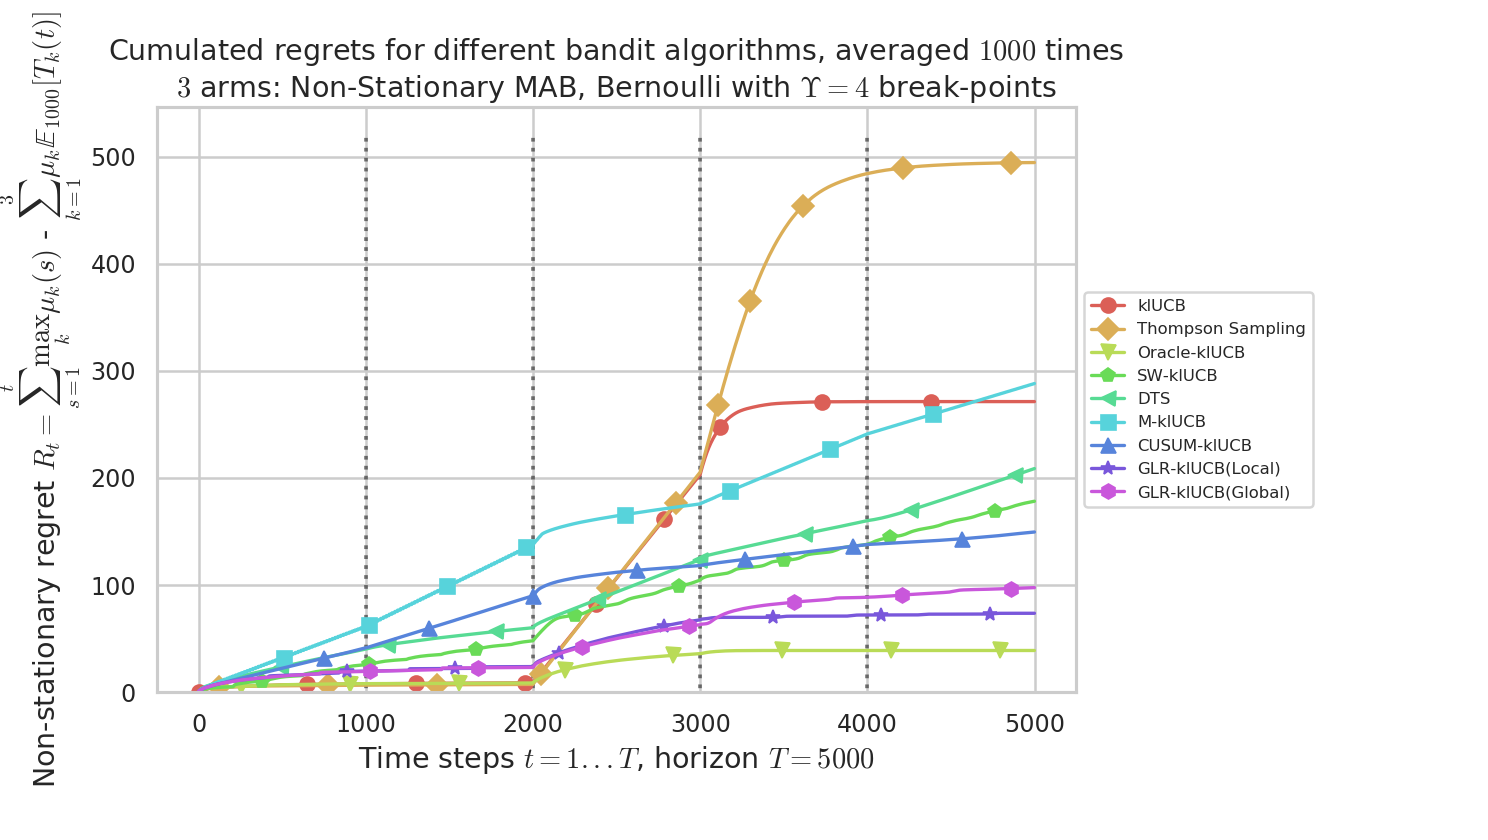
\includegraphics[width=1.15\textwidth]{figures/regret_problem1.png}
  $\implies$ BGLR achieves the best performance among non-oracle algorithms!
\end{frame}


\begin{frame}[plain]{Problem 2: only global changes}
  \centering
  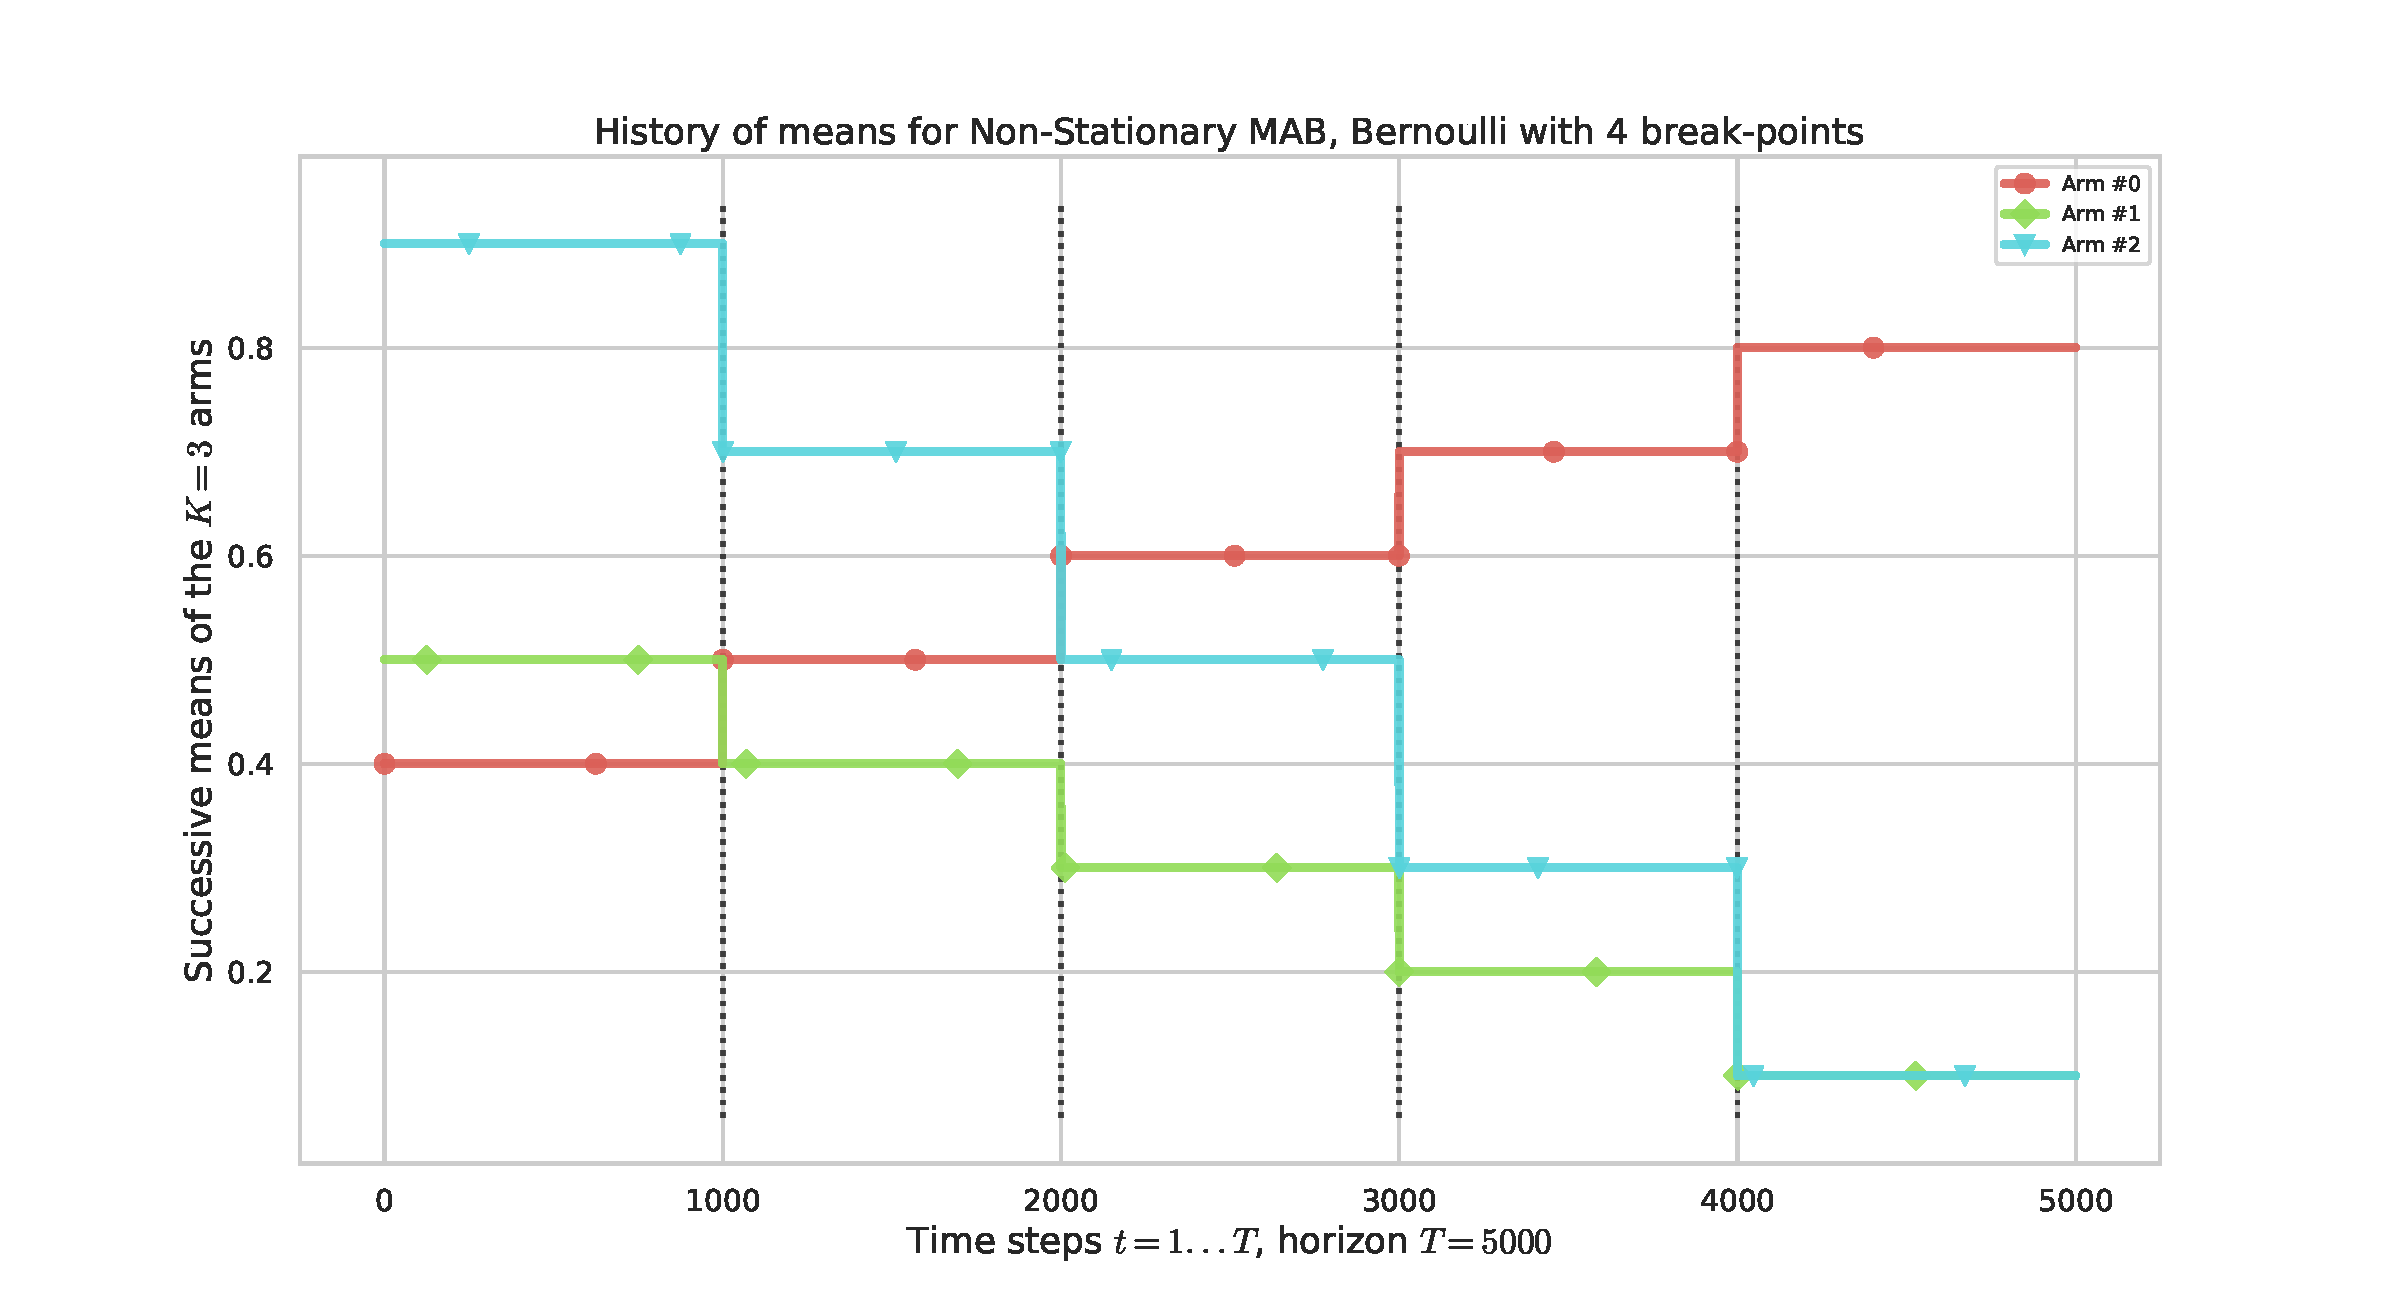
\includegraphics[width=1.00\textwidth]{figures/Problem_2.pdf}
\end{frame}

\begin{frame}[plain]{Results on problem 2}
  \centering
  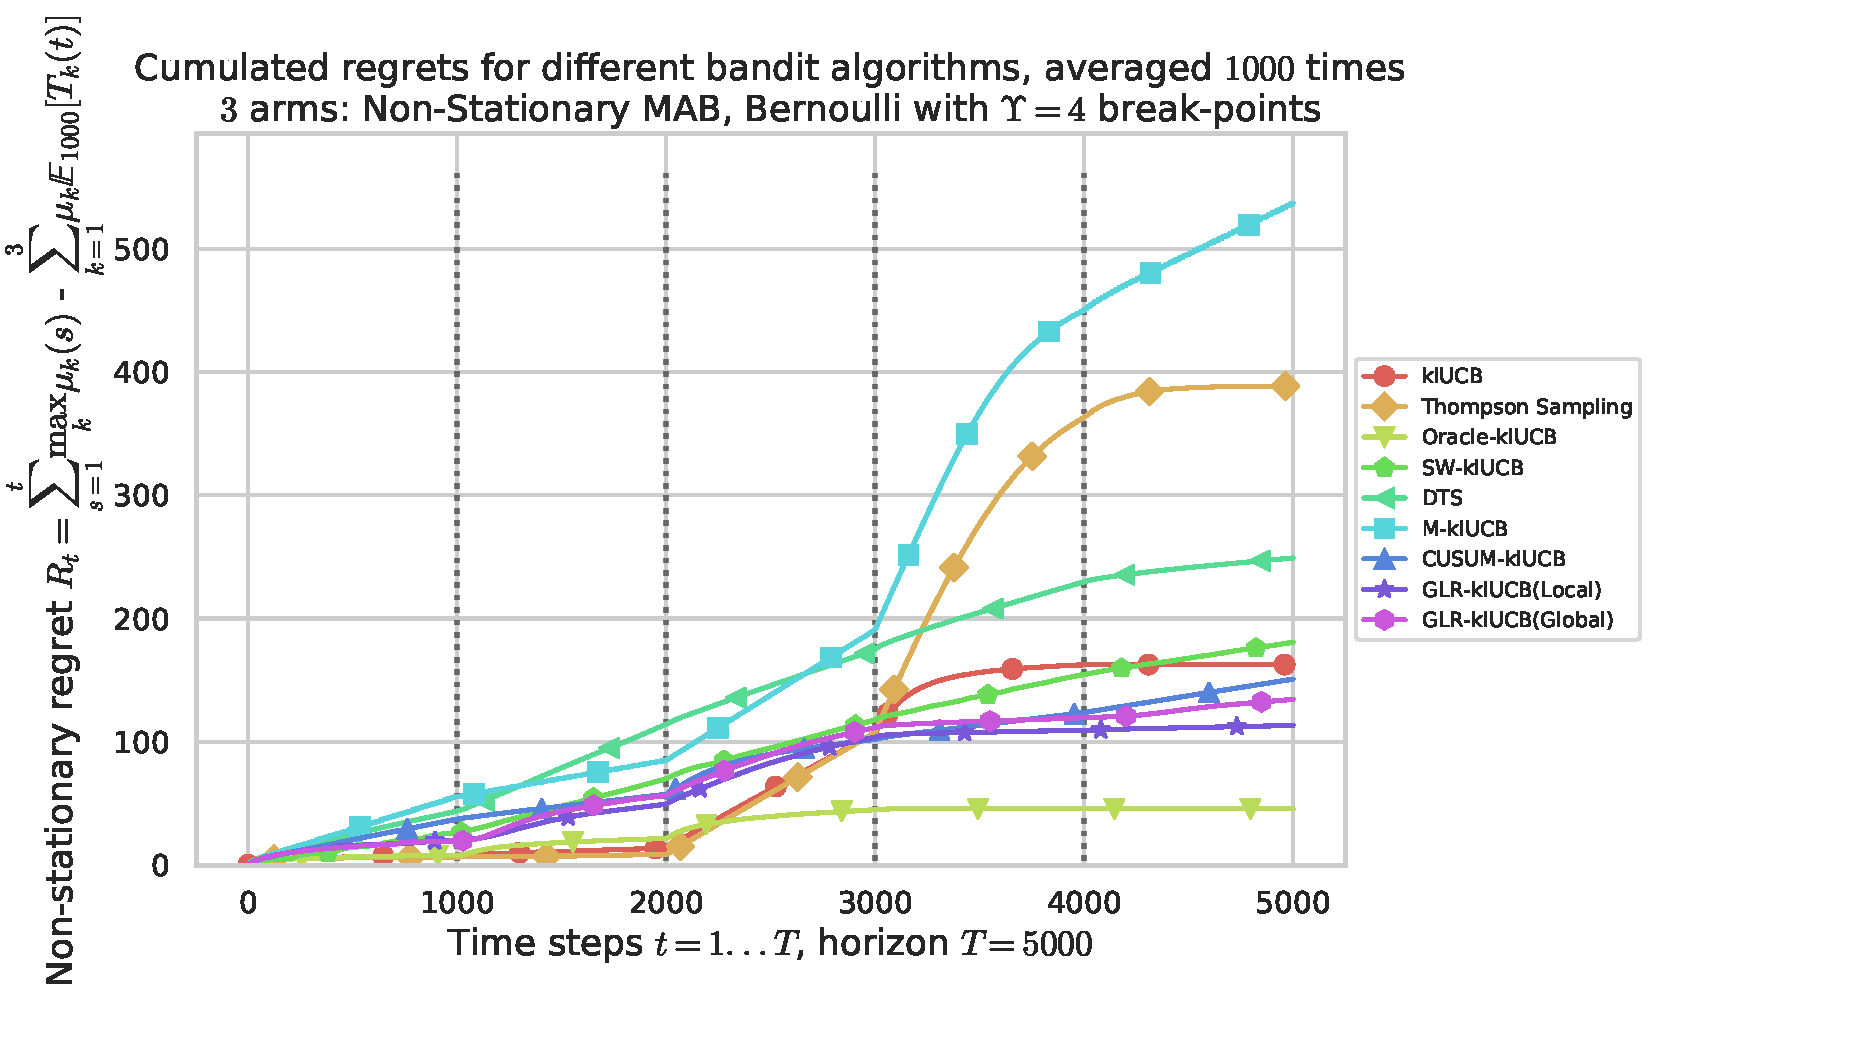
\includegraphics[width=1.15\textwidth]{figures/regret_problem2.pdf}
  $\implies$ BGLR again achieves the best performance!
\end{frame}


\begin{frame}[plain]{Pb 3: non-uniform lenghts of stationary sequences}
  \centering
  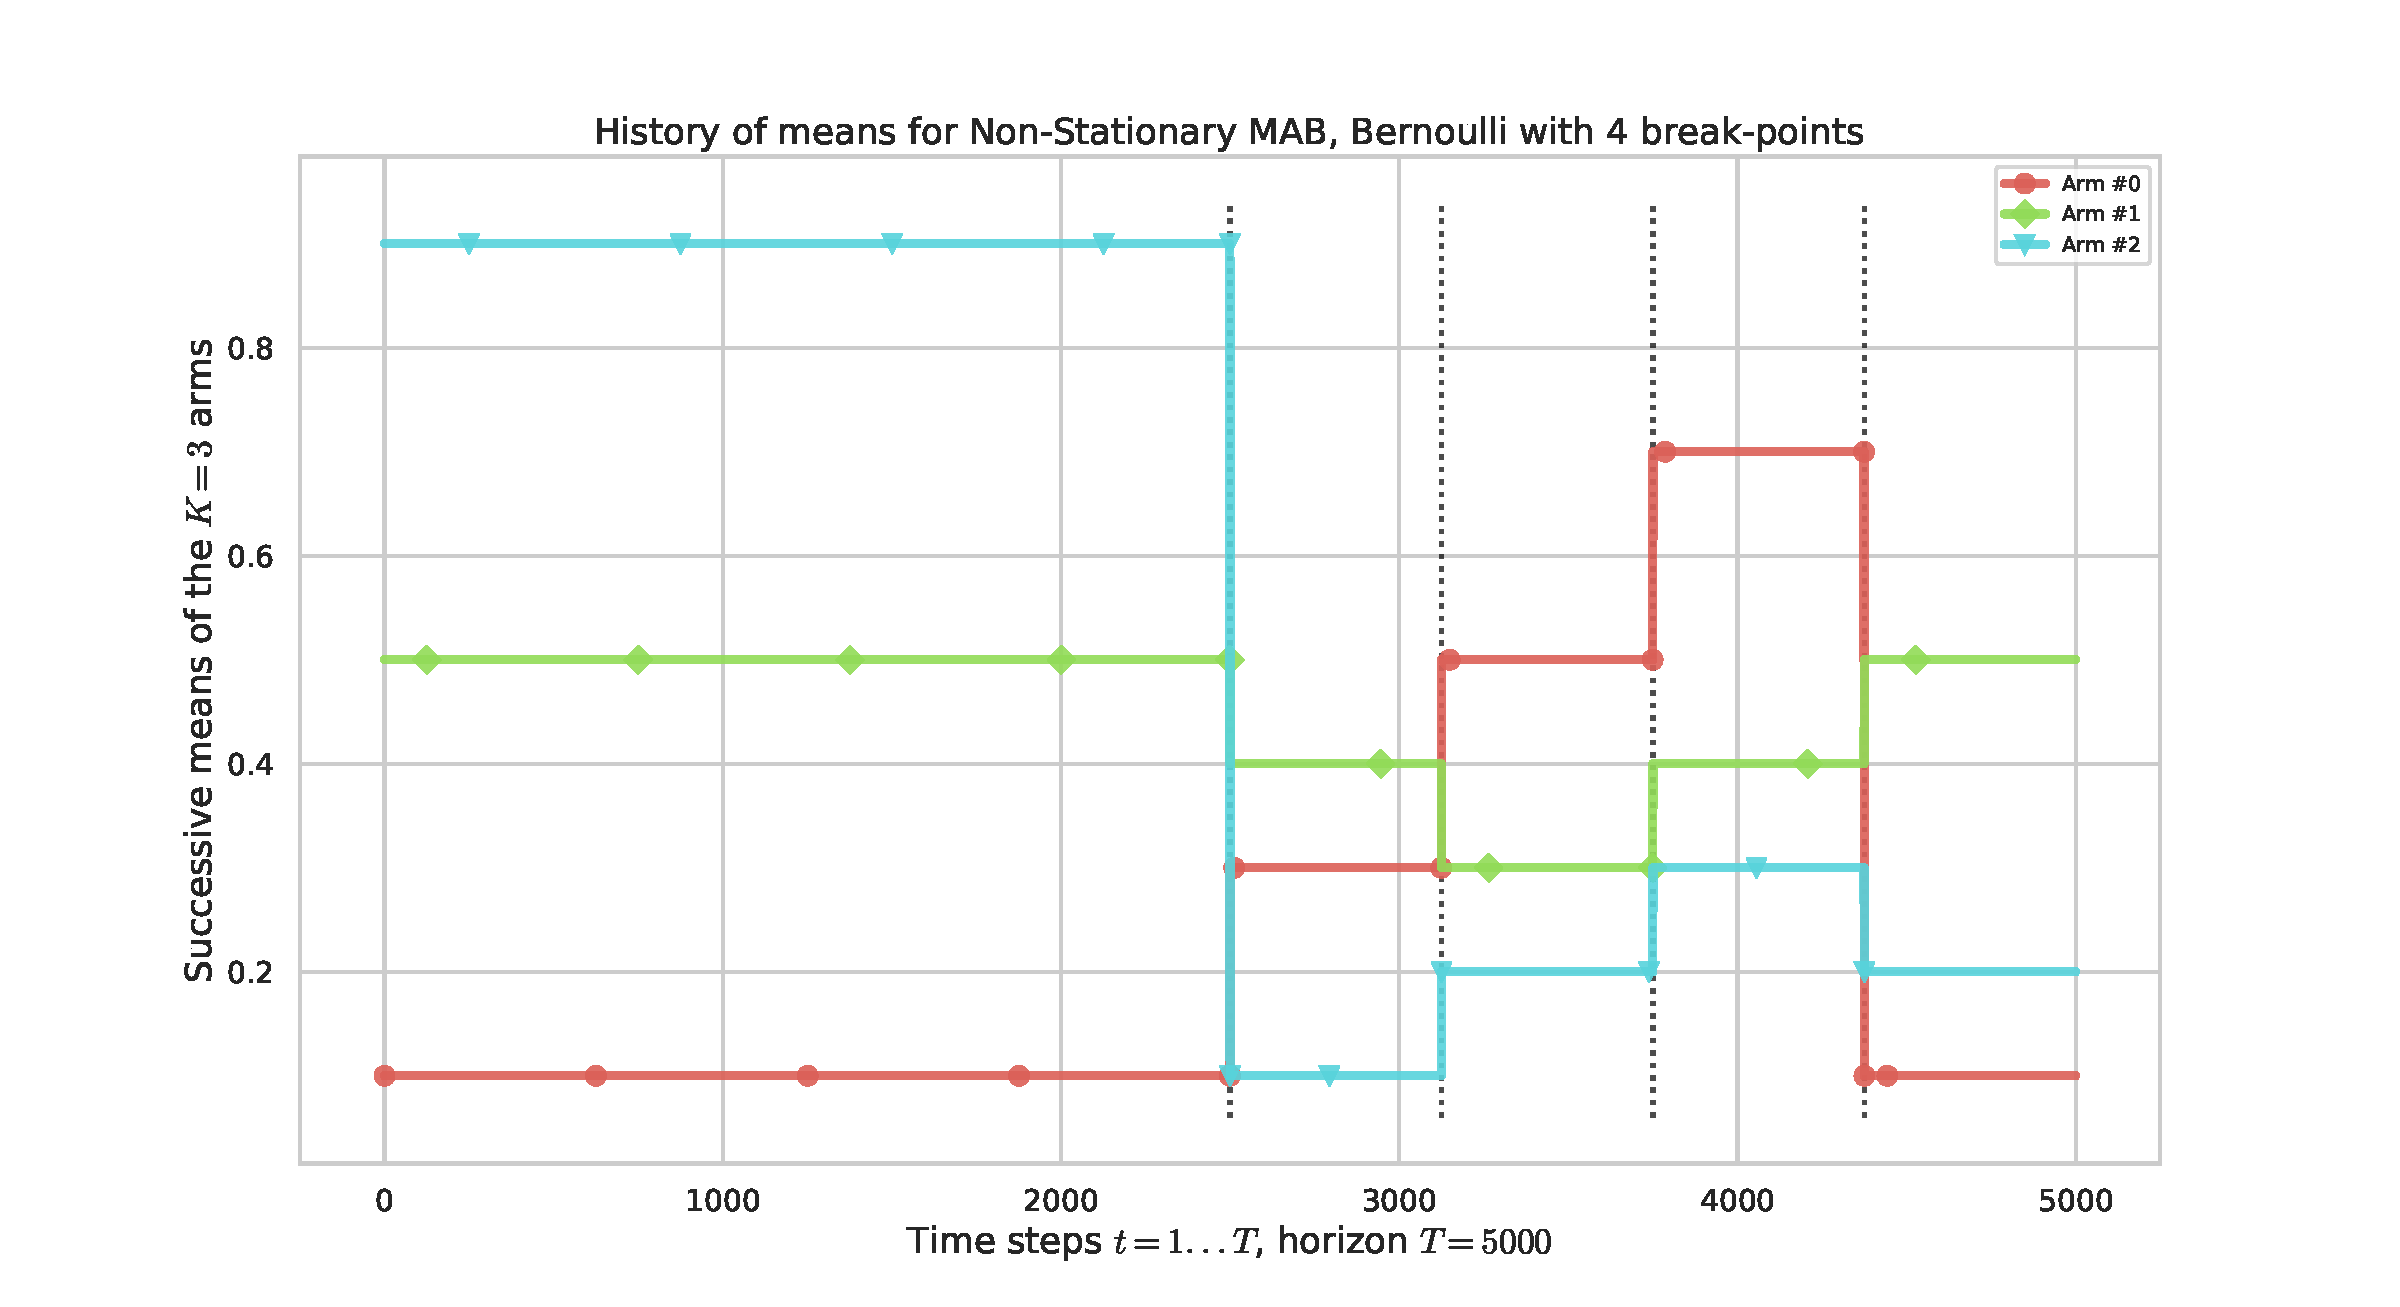
\includegraphics[width=1.00\textwidth]{figures/Problem_4.pdf}
\end{frame}

\begin{frame}[plain]{Results on problem 3}
  \centering
  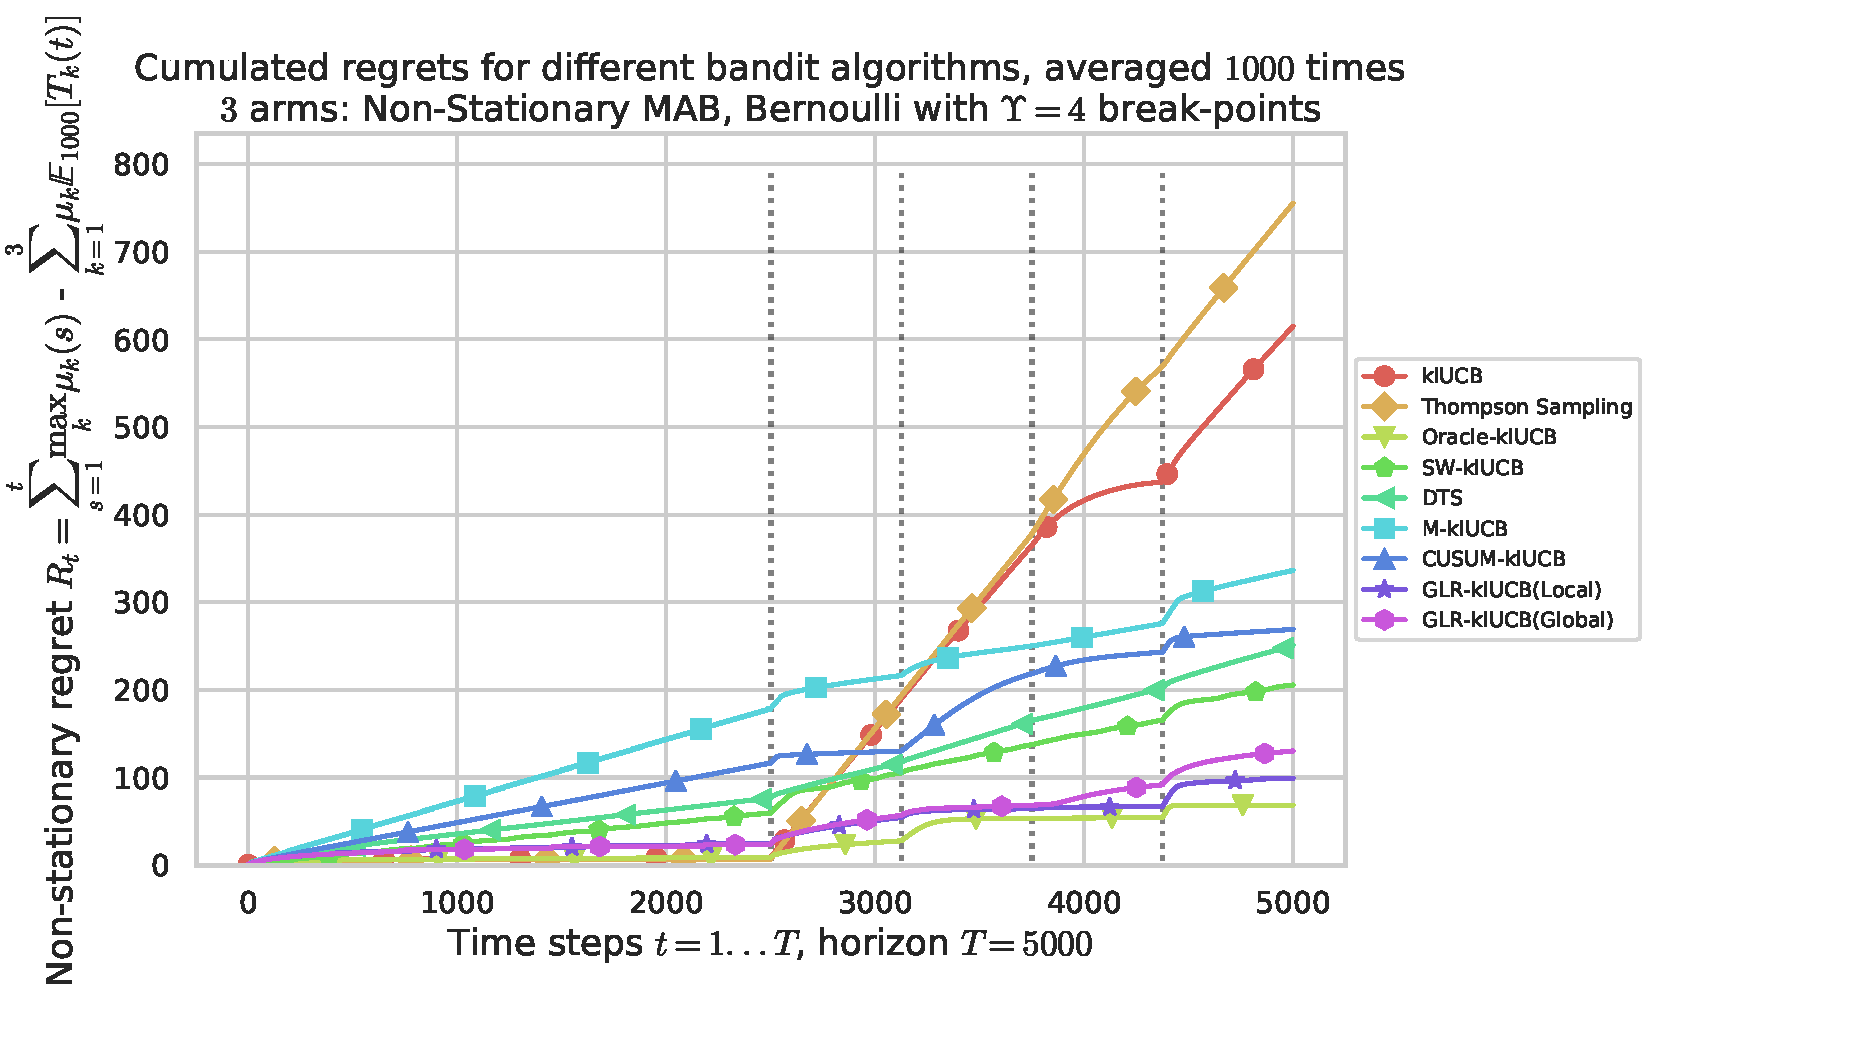
\includegraphics[width=1.15\textwidth]{figures/regret_problem4.pdf}
  $\implies$ BGLR achieves the best performance among non-oracle algorithms!
\end{frame}


\subsection{\hfill{}Conclusions from the simulations\hfill{}}

\begin{frame}{Interpretation of the simulations (1/2)}

  \begin{block}{Conclusions in terms of regret}
    \begin{itemize}
      \item
      Empirically we can check that the \alert{BGLR test is efficient}:
      \begin{itemize}\tightlist
        \item
        it has a \alert{low false alarm probability}
        \item
        it has a \alert{small delay} if the stationary sequences are long enough
      \end{itemize}
      And this is true even if the hypotheses of our analysis are not satisfied!
      \item
      Using the kl-UCB indexes policy gives good performance
    \end{itemize}
    $\implies$ Our algorithm (BGLR test + kl-UCB) is efficient

    $\implies$ We verified that it obtains state-of-the-art performance!
  \end{block}

\end{frame}


\begin{frame}{Interpretation of the simulations (2/2)}

  What about the efficiency in terms of time and memory?

  \begin{block}{Memory: efficient}
    Our algorithm is as efficient as other state-of-the-art strategies!\\
    Memory $= \mathcal{O}(K d_{\max})$
    for $K$ arms and horizon $T$.
  \end{block}

  \begin{alertblock}<2->{Time: slow!}
    But it is too slow!
    Time $= \mathcal{O}(K T d_{\max})$
    for $K$ arms and horizon $T$.

    $\hookrightarrow$ we proposed two numerical tweaks to speed it up

    $\implies$ BGLR test + kl-UCB can be as fast as M-UCB or CUSUM-UCB
    % , the two algorithms that perform as well in terms of regret

    $\hookrightarrow$  see the long version on \href{https://hal.inria.fr/hal-02006471}{\textcolor{blue}{HAL-02006471}} and \href{https://arxiv.org/abs/1902.01575}{\textcolor{blue}{arXiv:1902.01575}}
  \end{alertblock}

  ($d_{\max}$ $=$ duration of the longer stationary sequence, $T \leq (1+\Upsilon_T) d_{\max}$)

\end{frame}



\section{\hfill{}Conclusion\hfill{}}
\subsection{Summary}

\begin{frame}{Summary}

  What we just presented\ldots{}
  \begin{itemize}
    \item
    The Multi-Armed Bandits problem (MAB)
    \item
    Stationary, then \alert{piece-wise stationary}
    \item
    The BGLR test is efficient
    \begin{itemize}\tightlist
      \item
      to detect break-points with \alert{no false alarm} and \alert{low delay}
      \item
      for Bernoulli (or sub-Bernoulli) data,
      \item
      and does not need to know the amplitude of the break-point
    \end{itemize}
    \item
    We can combine it with an efficient MAB policy:
    \alert{BGLR + kl-UCB}
    \item
    Its regret bound is $R_T = \mathcal{O}(K \sqrt{T \Upsilon_T \log(T)})$ (state-of-the-art)
    \item
    On numerical simulations, our algorithm outperforms other efficient policies, and can be as fast as its best competitors
  \end{itemize}

\end{frame}

\subsection{Thanks}
\begin{frame}{Conclusion}

\begin{center}
  \begin{Large}
    {\Fontify Thanks for your attention .}
    \Smiley[0.9]
  \end{Large}
\end{center}

\vspace*{20pt}

\begin{center}
  \begin{Large}
    Questions \& Discussion ?
  \end{Large}
\end{center}

\end{frame}

\end{document}
